\section{Berechnung des \Gls{fahrtverlauf}s} \label{kapitelFahrtverlauf}
Der \Gls{fahrtverlauf} eines Fahrzeuges wird bei der Berechnung in zwei verschiedenen Arten gespeichert. Einmal in so genannten \textit{\$keyPoints}, welche in einem Array die Start- und Zielgeschwindigkeit (\textit{time\_0} und \textit{time\_0}), die Start- und Endposition (\textit{position\_0} und \textit{position\_1}) und die Start- und Endzeit (\textit{time\_0} und \textit{time\_1}) einer Beschleunigung bzw. Verzögerung abspeichern. Für die Überprüfung, ob ein Fahrzeug die zulässige Höchstgeschwindigkeit in einem Infrastrukturabschnitt überschreitet, für die spätere Übermittlung der \Gls{echtzeitdaten} an das Fahrzeug und die exakte Positionsbestimmung, werden mittels der \textit{\$keyPoints} für jede Geschwindigkeitsänderungen (und bei konstanter Geschwindigkeit in 1 Meter Abständen) die aktuelle relative Position innerhalb eines Infrastrukturabschnitts, der Infrastrukturabschnitt, die aktuelle Zeit und die aktuelle Geschwindigkeit in einem Array gespeichert.
Der \Gls{fahrtverlauf} wird mit der Funktion \textit{updateNextSpeed$($$)$} berechnet, welche als Parameter unter anderem die Zugdaten aus dem \textit{\$allUsedTrains}-Array, Start- und Endzeit der Fahrt (\textit{\$startTime} und \textit{\$endTime}), den Ziel-Infrastrukturabschnitt (\textit{\$targetSection}) und die relative Position in dem Ziel-Infrastrukturabschnitt (\textit{\$targetPosition}) übergeben bekommt.
Die für die Berechnung benötigten Daten werden in den in Tabelle \ref{table:vars} beschriebenen Variablen gespeichert.
\begin{table}
\begin{center}
\renewcommand{\arraystretch}{1.2}
\begin{tabular}{c|c}
Bezeichnung & Funktion \\ \hline
\textit{\$keyPoint} (Array)                   			&   \makecell{Beschreibt eine Beschleunigung bzw.\\Verzögerung (\textit{position\_0}, \textit{position\_1},\\ \textit{time\_0}, \textit{time\_1}, \textit{speed\_0}, \textit{speed\_1})}           \\ \hline
\textit{\$next\_section} (Array)                  		&    IDs aller Abschnitte                  \\ \hline
\textit{\$next\_lenghts} (Array)                  		&    Längen aller Abschnitte                  \\ \hline
\textit{\$next\_v\_max} (Array)                  		&    Höchstgeschwindigkeit aller Abschnitte                  \\ \hline
\textit{\$indexCurrentSection} (Integer)             	&    Index des aktuellen Abschnitts               \\ \hline
\textit{\$indexTargetSection} (Integer)               	&    Index des Ziel-Abschnitts                  \\ \hline
\textit{\$cumulativeSectionLengthStart} (Array) 	&    Absolute Startposition aller Abschnitte                  \\ \hline
\textit{\$cumulativeSectionLengthEnd} (Array)  	&    Absolute Endposition aller Abschnitte                  \\ \hline
\textit{\$trainPositionChange} (Array)                	&    Alle absoluten Positionen des \Gls{fahrtverlauf}s                  \\ \hline
\textit{\$trainSpeedChange} (Array)                  	&   Alle Geschwindigkeiten des \Gls{fahrtverlauf}s                  \\
\end{tabular}
\renewcommand{\arraystretch}{1}
\caption{Beschreibung der verwendeten Variablen für die Fahrtverlaufsberechnung}
\label{table:vars}
\end{center}
\end{table}
In dem folgenden Abschnitt werden die einzelnen Schritte beschrieben, die durchlaufen werden um den optimalen \Gls{fahrtverlauf} zu berechnen. In der Darstellung \ref{fig:fahrtverlauf} wird der Ablauf grob schematisch dargestellt.
\begin{center}
\begin{figure}
\centering
\begin{tikzpicture}[node distance=1cm, auto,]
\node[punkt] (a) {Berechnung bei einer Beschleunigung auf die maximal mögliche Geschwindigkeit};
\node[below=of a, punkt] (b) {Wird die Geschwindigkeit in Infrastrukturabschnitten überschritten?};
\node[right=of b, punkt](c) {Neuberechnung unter Berücksichtigung der Geschwindigkeitsüberschreitung};
\node[below=of b, punkt] (d) {Wird die Mindestzeit auf einer Geschwindigkeit eingehalten?};
\node[right=of d, punkt](e) {Neuberechnung unter Berücksichtigung der Mindestzeit auf einer Geschwindigkeit};
\node[below=of d, punkt] (f) {Erreicht der Fahrzeug mit einer Verspätung das Ziel?};
\node[right=of f, punkt] (g) {Kann die Geschwindigkeit reduziert werden, ohne dass das Fahrzeug eine Verspätung hat?};
\node[below=of f, punkt] (h) {Übermittlung der \Gls{echtzeitdaten} an das Fahrzeug};
\node[right=of g, punkt] (i) {Reduzierung der Geschwindigkeit unter Einhaltung der Ankunfrtszeit};
\node[right=of a, punkt] (j) {Ist eine Fahrt ohne Gefahrenbremsung möglich?};
\node[right=of j, punkt] (k) {Berechnung der Gefahrenbremsung};
\node[above=of j, punkt] (l) {Start der Fahrtverlaufsberechnung};
\draw [pil] (a) -- (b);
\draw [pil] (b) --  node[pos=0.5] {Ja} (c);
\draw [pil] (c.north) -- +(0,0.5) -|  (b.north); 
\draw [pil] (b) -- node[pos=0.5,left] {Nein} (d);
\draw [pil] (d) --  node[pos=0.5] {Nein} (e);
\draw [pil] (e.north) -- +(0,0.3) -|  (d.north); 
\draw [pil] (d) -- node[pos=0.5,left] {Ja} (f);
\draw [pil] (f) -- node[pos=0.5] {Ja} (g);
\draw [pil] (f) -- node[pos=0.5,left] {Nein} (h);
\draw [pil] (g) -- node[pos=0.5] {Ja} (i);
\draw [pil] (g.south) -- node[pos=0.5,left] {Nein} +(0,-1) |-  (h.east); 
\draw [pil] (i.south) -- +(0,-1) |-  (h.east); 
\draw [pil] (j) -- node[pos=0.5,above] {Ja} (a);
\draw [pil] (j) -- node[pos=0.5] {Nein} (k);
\draw [pil] (l) -- (j);
\draw [pil] (k.east) -- +(0.5,0) |- (h.east);
\end{tikzpicture}
\caption{Ablaufplan der Fahrtverlaufsberechnung}
\label{fig:fahrtverlauf}
\end{figure}
\end{center}
\subsection{Ermittlung der Start- und Endposition der einzelnen Infrastrukturabschnitte unter Berücksichtigung der Zuglänge}
Für die Berechnung eines exemplarischen \Gls{fahrtverlauf}s wurden die in Tabelle \ref{table:infraex} definierten Infrastrukturabschnitte benutzt. Diese Abschnitte wurden so gewählt, sodass alle Funktionen und die Allgemeingültigkeit des Algorithmus gezeigt werden können und treten so im \ac{ebuef} nicht auf. 
\begin{table}
\begin{center}
\renewcommand{\arraystretch}{1.2}
\begin{tabular}{c| C{3cm} |c}
Infrastrukturabschnitts-ID & Länge & zulässige Höchstgeschwindigkeit \\ \hline
1000                   &   300 $m$    & 120 $km/h$                        \\ \hline
1001                  &    400 $m$   & 120 $km/h$                        \\ \hline
1002                   &   300 $m$    &        120 $km/h$                         \\ \hline
1003                   &    400 $m$   &         90 $km/h$                        \\ \hline
1004                   &    300 $m$   &            60 $km/h$                     \\ \hline
1005                   &   200 $m$    &           60 $km/h$                      \\ \hline
1006                   &  400 $m$     &      90 $km/h$                           \\ \hline
1007                   &  500 $m$     &      120 $km/h$                           \\ \hline
1008                   &   300 $m$    &      120 $km/h$                           \\ \hline
1009                   &   400 $m$    &      100 $km/h$                           \\ \hline
1010                   &   300 $m$    &      60 $km/h$                           \\ \hline
1011                   &   300 $m$    &         40 $km/h$                        \\ 
\end{tabular}
\renewcommand{\arraystretch}{1}
\caption{Exemplarische Infrastrukturabschnitte}
\label{table:infraex}
\end{center}
\end{table}
Als exemplarisch gewählte Zugdaten wurden die in Tabelle \ref{table:train-ex} definierten Daten verwendet.
\begin{table}[]
\begin{center}
\renewcommand{\arraystretch}{1.2}
\begin{tabular}{r L{3cm}}
relative Startposition                   &   10 $m$                         \\ 
relative Zielposition                  &    290 $m$                         \\ 
aktueller Infrastrukturabschnitt                   &   1001                         \\ 
Ziel-Infrastrukturabschnitt                  &    1010                         \\ 
Startgeschwindigkeit                   &   0 $km/h$                          \\ 
Zielgeschwindigkeit                   &    0 $km/h$                        \\ 
Zuglänge                   &    50 $m$                        \\ 
Bremsverzögerung                   &    0,8 $m/s^{2}$                        \\ 
Fahrplan vorhanden                   &    ja                        \\ 
Zeit bis zur nächsten Betriebsstelle                   &    210 $s$                        \\ 
\end{tabular}
\renewcommand{\arraystretch}{1}
\caption{Exemplarische Zugdaten}
\label{table:train-ex}
\end{center}
\end{table}
Die zuvor ermittelten nächsten Infrastrukturabschnitte inklusive derer Längen und zulässigen Höchstgeschwindigkeit müssen für die Berechnung des \Gls{fahrtverlauf}s angepasst werden, da ein Fahrzeug erst beschleunigen darf, wenn das komplette Fahrzeug in den Infrastrukturabschnitt eingefahren ist. In Darstellung \ref{fig:it1} sind die Infrastrukturabschnitte dargestellt, so wie sie von dem Fahrzeug ermittelt wurden. Dabei werden alle Abschnitte, die das Fahrzeug schon durchfahren hat oder hinter dem Zielabschnitt liegen nicht dargestellt. Zudem wird in dem aktuellen Abshcnitt die relative Position von der Länge abgezogen und in der Zielabschnitt wird nur bis zur relativen Zielposition abgebildet. Dementsprechend ist der erste Abschnitt in der Darstellung \ref{fig:it1} der Abschnitt mit der ID 1001. Dieser hat aufgrund der aktuellen relativen Position des Fahrzeugs eine Länge von 290 $m$. Und der letzte Abschnitt ist der Abschnitt mit der ID 1010 und einer Länge von ebenfalls 290 $m$.
\begin{figure}
  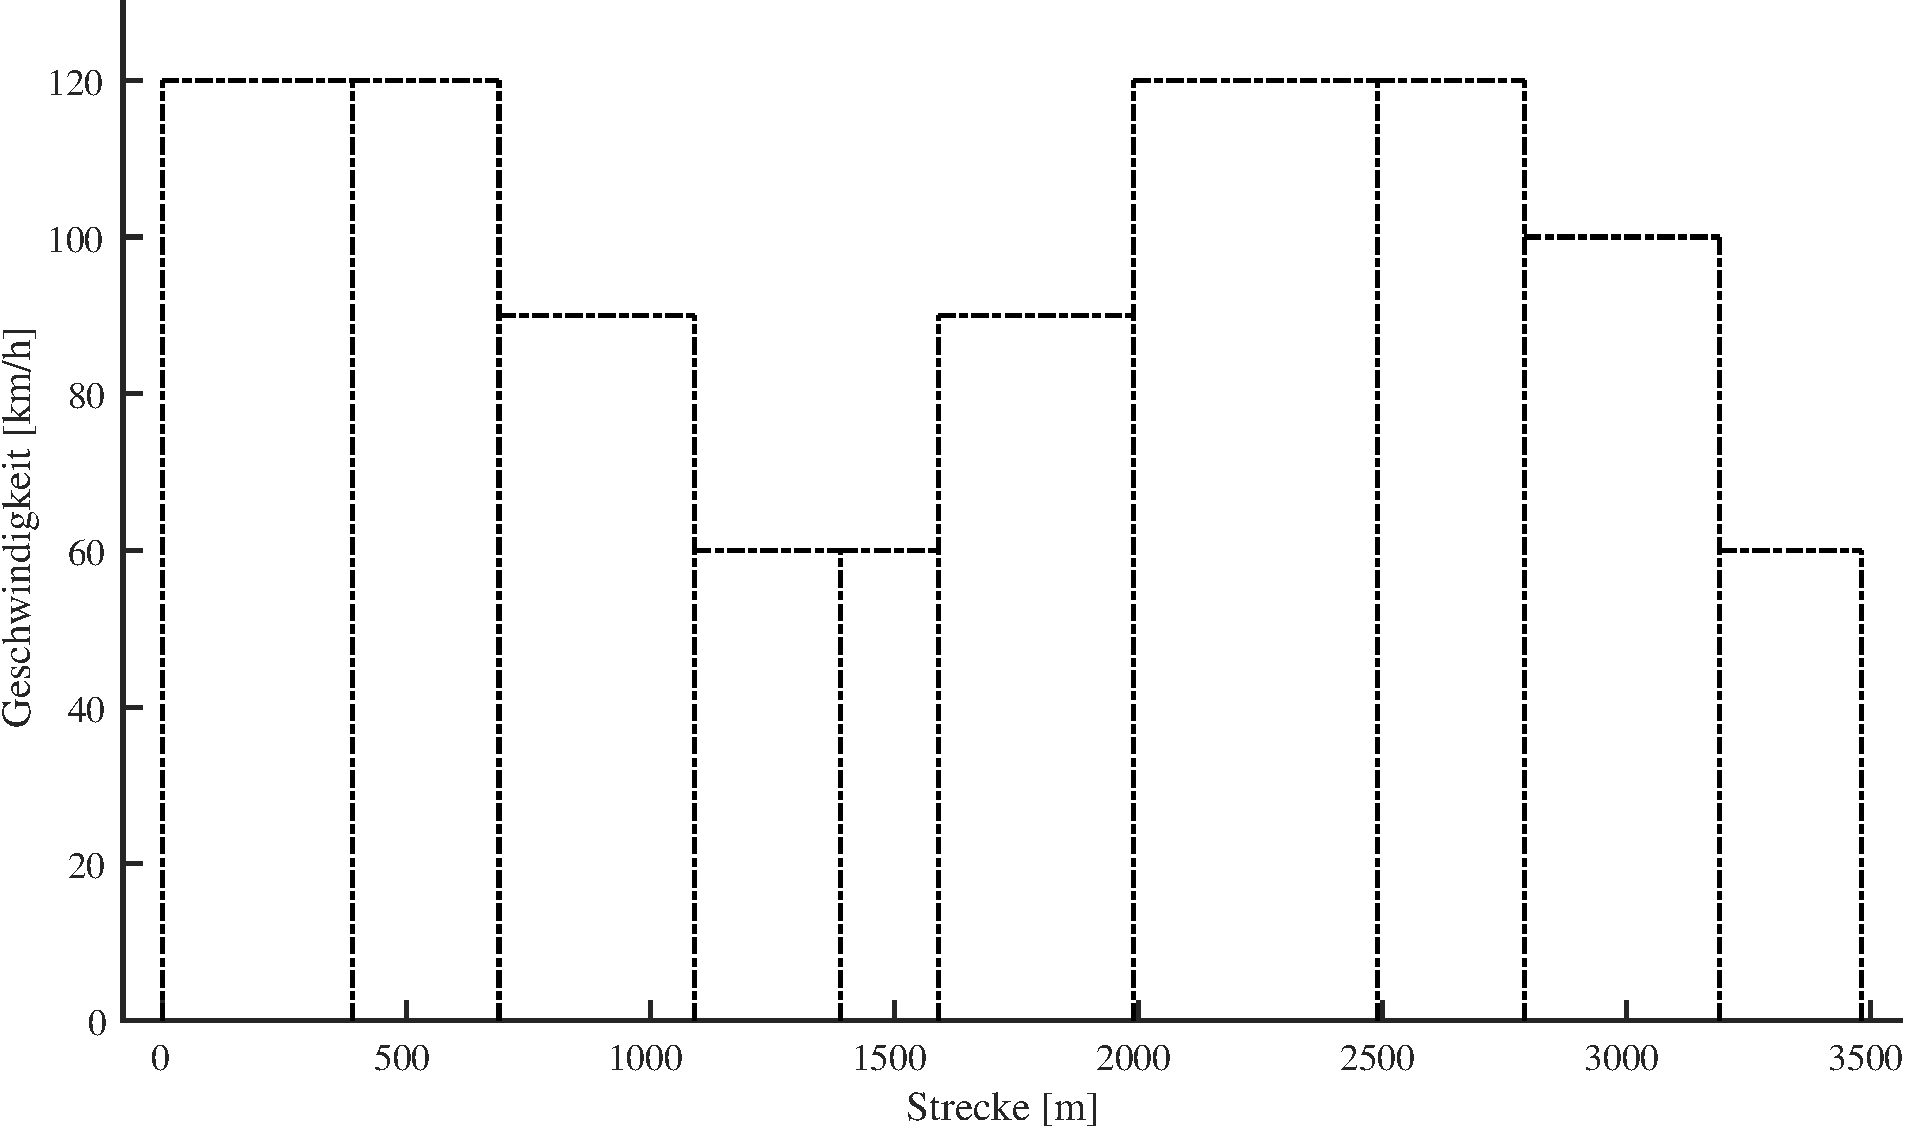
\includegraphics[width=\linewidth]{../images/matlab/it1.pdf}
  \caption{Darstellung der Infrastrukturabschnitte und die zugehörige Höchstgeschwindigkeit}
  \label{fig:it1}
\end{figure}
Bei der Berücksichtigung der Fahrzeuglänge wird durch alle Infrastrukturabschnitt iteriert und die Zuglänge auf die Länge das Abschnitts addiert. Von dieser neu ermittelten Endposition des Abschnitts wird überprüft, ob zwischen der vorherigen Endposition und der neu ermittelten Endposition ein Infrastrukturabschnitt liegt, dessen zulässige Höchstgeschwindigkeit geringer ist, als die des ursprünglichen Abschnitts. Wenn dieser Fall eintritt, wird der Abschnitt nur so weit verlängert, sodass keine Höchstgeschwindigkeit der folgenden Abschnitte überschritten wird. Von der neu ermittelten Endposition wird überprüft, in welchem Abschnitt diese liegt und mit dem Abschnitt wird dann weiter gerechnet. Sobald der Ziel-Abschnitt erreicht wurde, wird die Schleife abgebrochen. Die neu ermittelten Abschnitte werden in den Arrays \textit{\$next\_lengths\_mod} und \textit{\$next\_v\_max\_mod} abgespeichert. Durch diese Algorithmus kann es dazu kommen, dass sich die Anzahl der Abschnitte verändert hat. Dementsprechend können die Abschnitte nicht mehr eindeutig mit der Infrastruktur-ID bezeichnet werden. Mittels \textit{\$next\_lengths\_mod} und \textit{\$next\_v\_max\_mod} werden mit der Funktion \textit{createCumulativeSections$($$)$} für jeden Abschnitt die absolute Start- und Endposition in den Arrays \textit{\$cumulativeSectionLengthStartMod} und \textit{\$cumulativeSectionLengthEndMod} gespeichert. Diese Umwandlung ist essentiell für die Überprüfung, in welchem Abschnitt ein Fahrzeug sich aktuell befindet. Die neu berechneten Abschnitte werden sind in der Darstellung \ref{fig:it2} in rot abgebildet und beschreiben die maximale Geschwindigkeit, die ein Fahrzeug fahren darf an der jeweiligen Position.
\begin{figure}
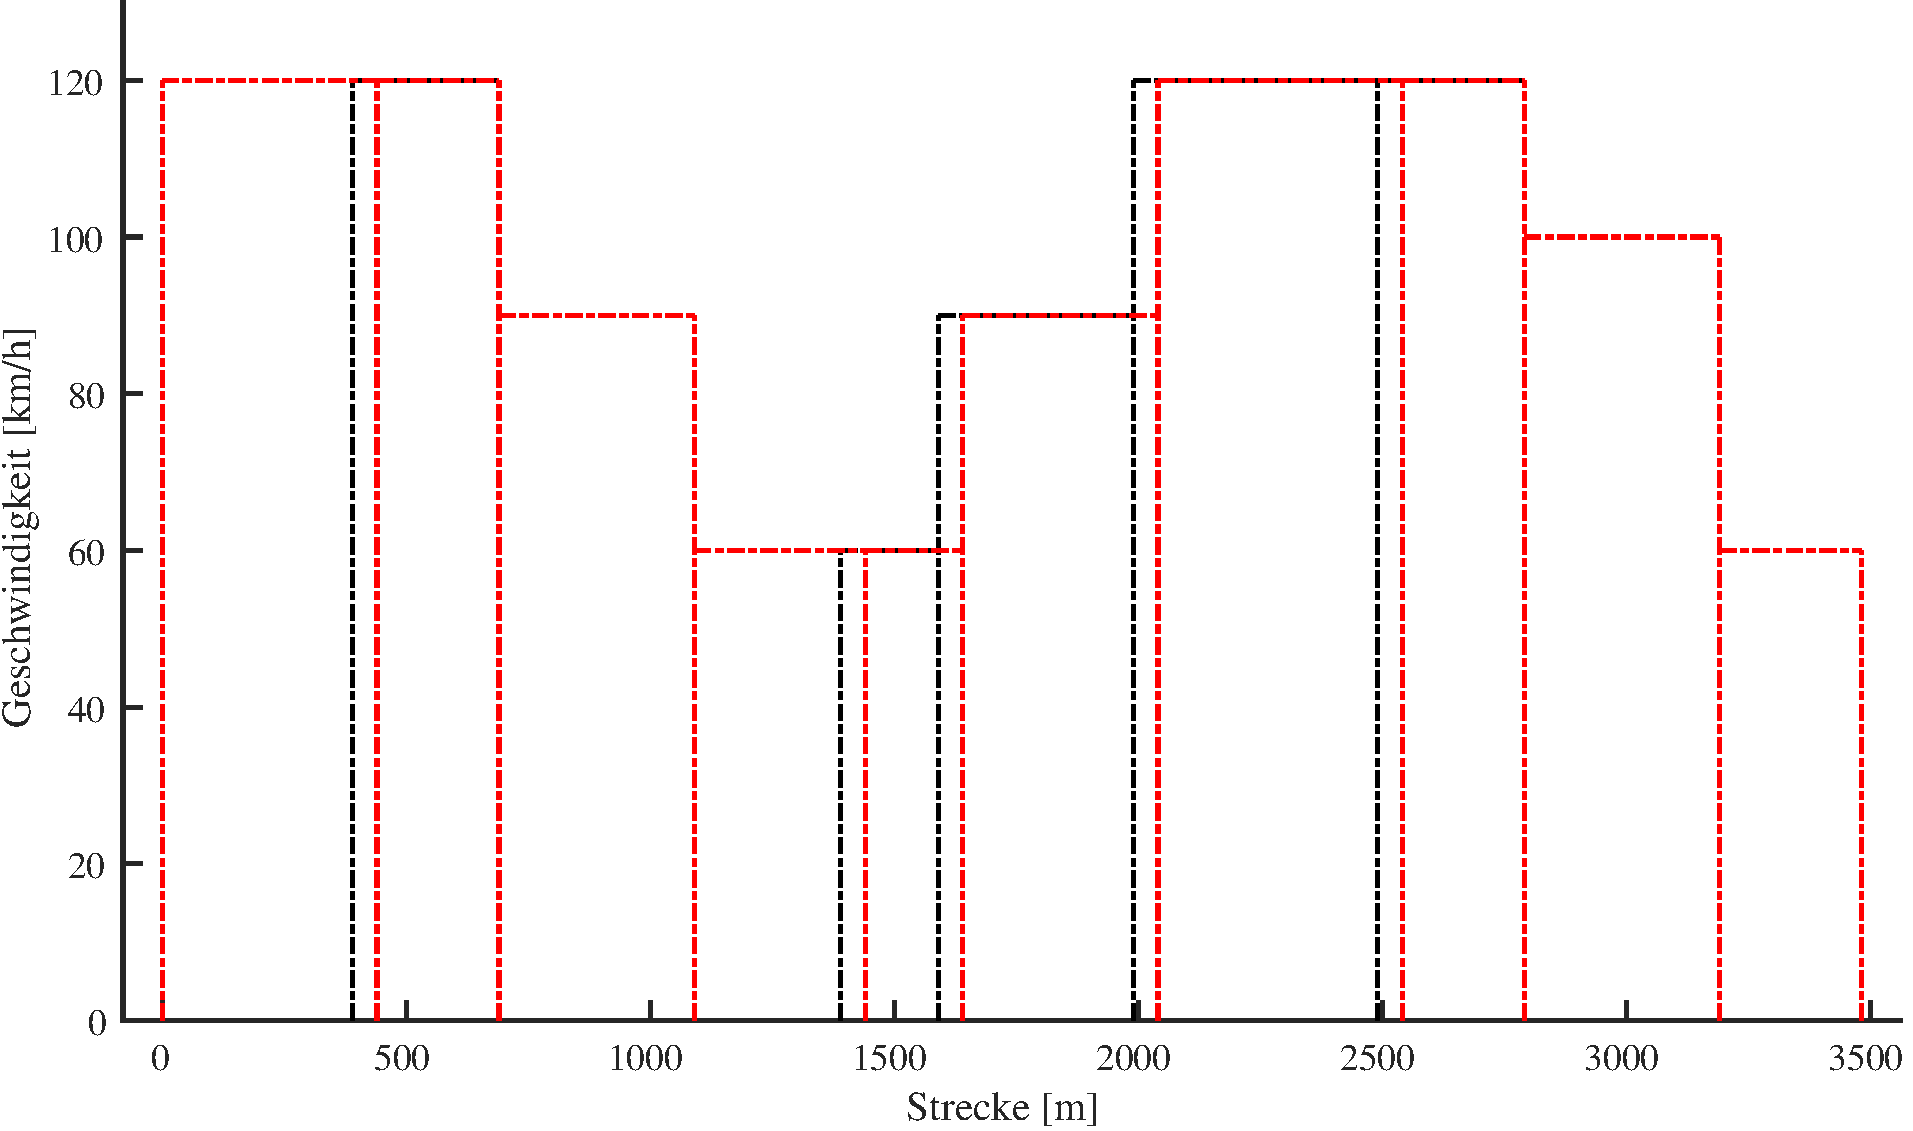
\includegraphics[width=\linewidth]{../images/matlab/it2.pdf}
\caption{Darstellung Infrastrukturabschnitte und die zugehörige Höchstgeschwindigkeit unter Berücksichtigung der Fahrzeuglänge}
\label{fig:it2}
\end{figure}
\subsection{Berechnung bei einer Beschleunigung auf die maximal mögliche Geschwindigkeit} \label{v_max}
Im ersten Schritt für die Distanz zwischen der aktuellen Position und der Ziel-Position mittels \textit{\$cumulativeSectionLengthStart}, \textit{\$cumulativeSectionLengthEnd}, \textit{\$indexCurrentSection} und \textit{\$indexTargetSection} berechnet. Für diese Distanz und die Startgeschwindigkeit wird mit Hilfe der Funktion \textit{getVMaxBetweenTwoPoints$($$)$} (Code-Beispiel ~\ref{lst:getVMaxBetweenTwoPoints}) die maximale Geschwindigkeit ermittelt, die das Fahrzeug aufnehmen kann, um noch bis zum Ziel rechtzeitig bremsen zu können. Dabei wird in 10 $km/h$-Schritten iteriert und der maximale Wert zurückgegeben. Innerhalb der Funktion wir die Funktion \textit{getBrakeDistance$($$)$} (Code-Beispiel ~\ref{lst:getBrakeDistance}) aufgerufen, welche die benötigte Distanz für eine Beschleunigung bzw. Verzögerung berechnet. 
\begin{figure}
\begin{lstlisting}[caption={\textit{getVMaxBetweenTwoPoints$($$)$}},captionpos=b,label={lst:getVMaxBetweenTwoPoints}]
function getVMaxBetweenTwoPoints(float $distance, int $v_0, int $v_1) {
	global $verzoegerung;
	global $globalFloatingPointNumbersRoundingError;
	$v_max = array();
	for ($i = 0; $i <= 120; $i = $i + 10) {
		if ((getBrakeDistance($v_0, $i, $verzoegerung) + getBrakeDistance($i, $v_1, $verzoegerung)) < ($distance + $globalFloatingPointNumbersRoundingError)) {
			array_push($v_max, $i);
		}
	}
	if (sizeof($v_max) == 0) {
		if ($v_0 == 0 && $v_1 == 0 && $distance > 0) {
			echo "Der zug müsste langsamer als 10 km/h fahren, um das Ziel zu erreichen.";
		} else {
			// TODO: Notbremsung
		}
	} else {
		if ($v_0 == $v_1 && max($v_max) < $v_0) {
			$v_max = array($v_0);
		}
	}
	return max($v_max);
}
\end{lstlisting}
\end{figure}
\begin{figure}
\begin{lstlisting}[caption={\textit{getBrakeDistance$($$)$}},captionpos=b,label={lst:getBrakeDistance}]
function getBrakeDistance (float $v_0, float $v_1, float $verzoegerung) {
	if ($v_0 > $v_1) {
		return $bremsweg = 0.5 * ((pow($v_0/3.6,2)-pow($v_1/3.6, 2))/($verzoegerung));
	} if ($v_0 < $v_1) {
		return $bremsweg = -0.5 * ((pow($v_0/3.6,2)-pow($v_1/3.6, 2))/($verzoegerung));
	} else {
		return 0;
	}
}
\end{lstlisting}
\end{figure}
Durch die gegebene Startgeschwindigkeit und die höchstmögliche Geschwindigkeit wird ein erster \Gls{fahrtverlauf} berechnet. Dabei werden zwei \textit{\$keyPoints} erzeugt. Mithilfe der Funktion \textit{createTrainChanges$($$)$} wird aus diesen beiden \textit{\$keyPoints} für jede Geschwindigkeitsveränderung die aktuelle absolute Position und Geschwindigkeit ermittelt. An den Positionen, an den das Fahrzeug eine konstante Geschwindigkeit hat, wird in 1 Meter Abständen die absolute Position und die Geschwindigkeit gespeichert. Die ermittelten Daten werden in den Arrays \textit{\$trainPositionChange} und \textit{\$trainSpeedChange} gespeichert. In der Darstellung \ref{fig:it3} ist das Ergebnis der 1. Iteration abgebildet.
\begin{figure}
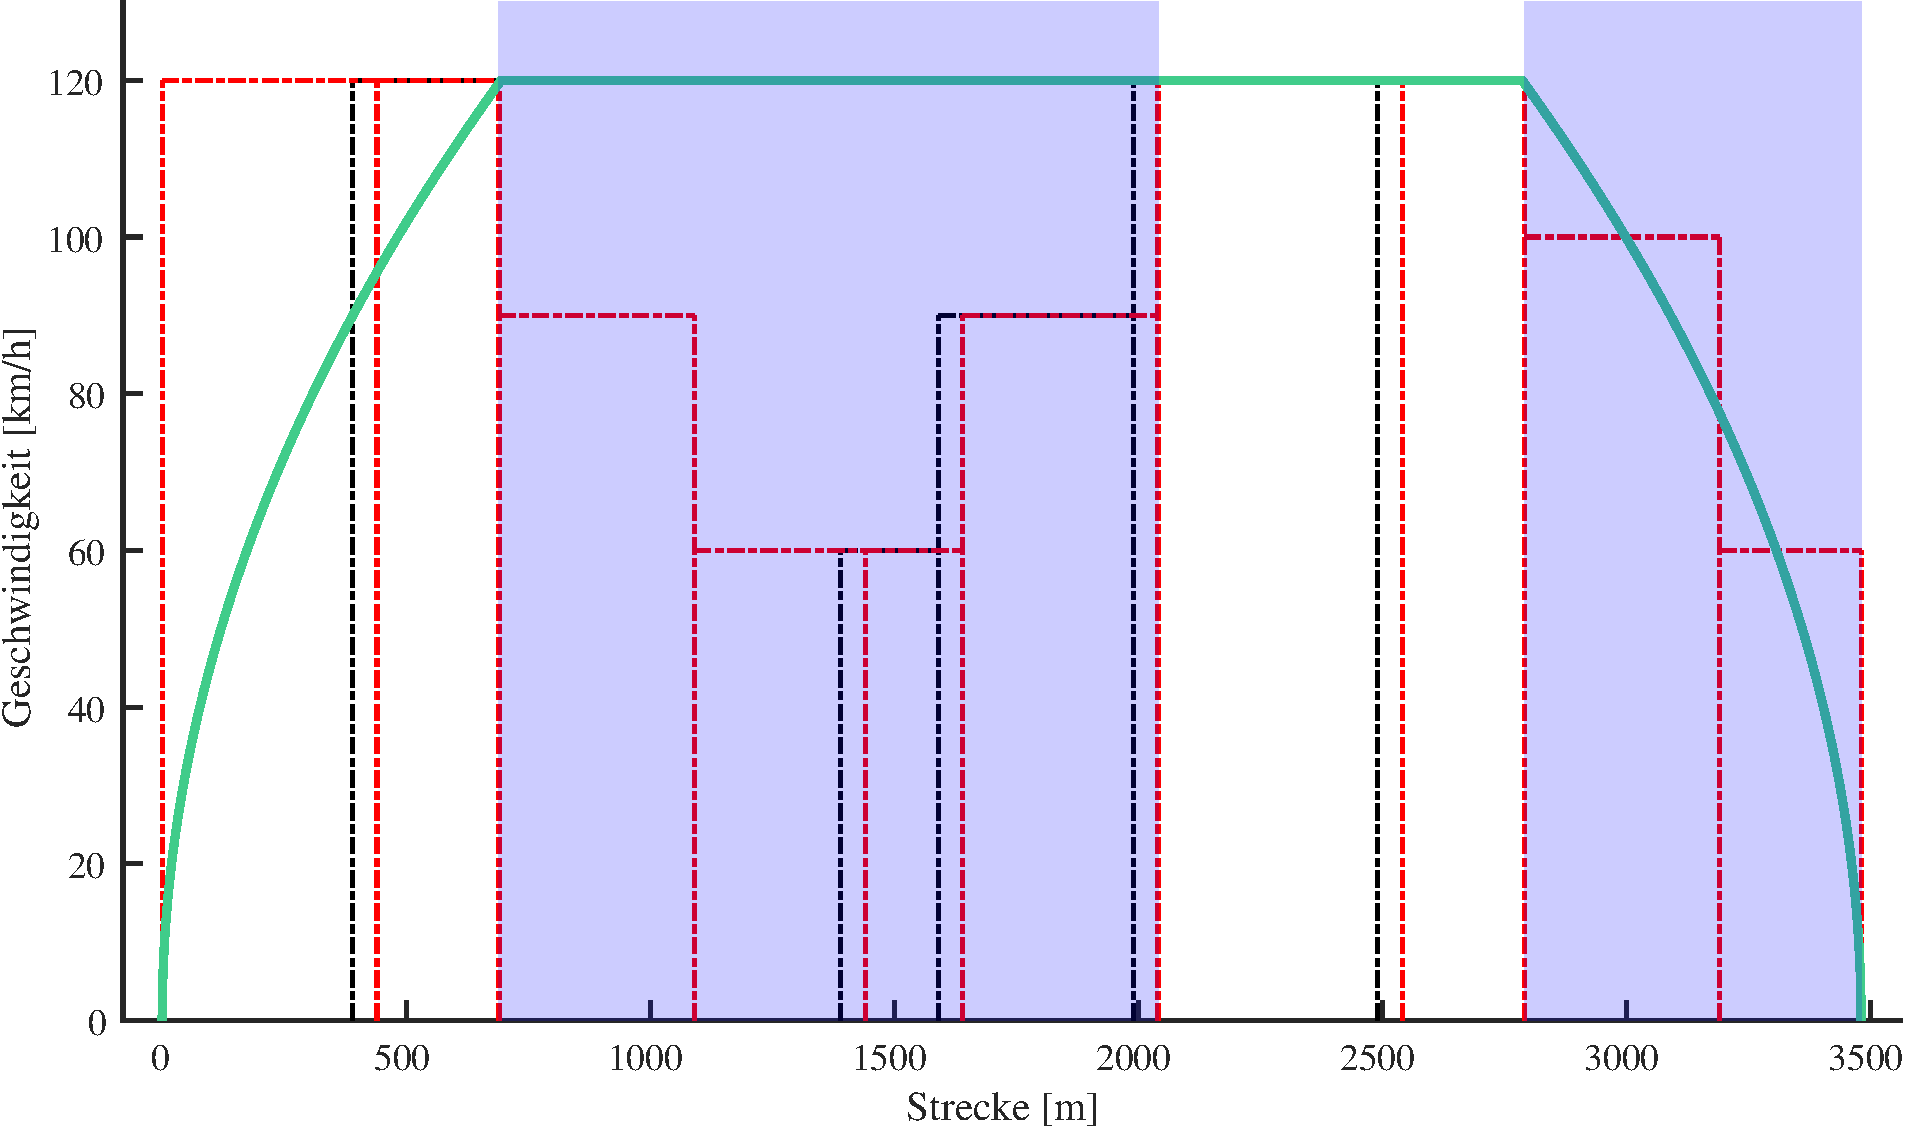
\includegraphics[width=\linewidth]{../images/matlab/it3.pdf}
\caption{Fahrtverlaufberechnung (1. Iteration)}
\label{fig:it3}
\end{figure}
\subsection{Überprüfung des \Gls{fahrtverlauf}s nach Geschwindigkeitsüberschreitungen} \label{überprüfung}
Für die Überprüfung, ob bei einem \Gls{fahrtverlauf} in manchen Infrastrukturabschnitten die zulässige Höchstgeschwindigkeit überschritten wird, wird nach jeder Berechnung die Funktion \textit{checkIfTrainIsToFastInCertainSections$($$)$} (Code-Beispiel ~\ref{lst:checkIfTrainIsToFastInCertainSections}) aufgerufen. In dieser Funktion wird über alle absoluten Positionen (\textit{\$trainPositionChange}) iteriert, überprüft in welchem Abschnitt sich diese Position befindet und überprüft, ob die zugehörige Geschwindigkeit aus dem \textit{\$trainSpeedChange}-Array die zulässige Höchstgeschwindigkeit überschreitet. Sobald in einem Abschnitt eine Geschwindigkeitsüberschreitung vorliegt, wird der zugehörige Index des Abschnitts in dem \textit{\$faildSections}-Array gespeichert. Diese Abschnitte sind in der Darstellung \ref{fig:it3} Lila hinterlegt. Als Rückgabewert der Funktion wird wird ein Array wiedergegeben, welches abspeichert, ob es zu einer Geschwindigkeitsüberschreitung gekommen ist (\textit{\grqq{}failed\grqq{}}) und wenn das der Fall ist auch die Indexe der Abschnitte (\textit{\grqq{}failed\_sections\grqq{}}).
\begin{figure}
\begin{lstlisting}[caption={\textit{checkIfTrainIsToFastInCertainSections$($$)$}},captionpos=b,label={lst:checkIfTrainIsToFastInCertainSections}]
function checkIfTrainIsToFastInCertainSections() {
	global $trainPositionChange;
	global $trainSpeedChange;
	global $cumulativeSectionLengthStartMod;
	global $next_v_max_mod;
	global $indexTargetSectionMod;
	$faildSections = array();
	foreach ($trainPositionChange as $trainPositionChangeKey => $trainPositionChangeValue) {
		foreach ($cumulativeSectionLengthStartMod as $cumulativeSectionLengthStartKey => $cumulativeSectionLengthStartValue) {
			if ($trainPositionChangeValue < $cumulativeSectionLengthStartValue) {
				if ($trainSpeedChange[$trainPositionChangeKey] > $next_v_max_mod[$cumulativeSectionLengthStartKey - 1]) {
					array_push($faildSections, ($cumulativeSectionLengthStartKey -1));
				}
				break;
			} else if ($cumulativeSectionLengthStartKey == $indexTargetSectionMod) {
				if ($trainPositionChangeValue > $cumulativeSectionLengthStartValue) {
					if ($trainSpeedChange[$trainPositionChangeKey] > $next_v_max_mod[$cumulativeSectionLengthStartKey]) {
						array_push($faildSections, $cumulativeSectionLengthStartKey);
					}
					break;
				}
			}
		}
	}
	if (sizeof($faildSections) == 0) {
		return array("failed" => false);
	} else {
		return array("failed" => true, "failed_sections" => array_unique($faildSections));
	}
}
\end{lstlisting}
\end{figure}
\subsection{Neuberechnung unter Berücksichtigung der Geschwindigkeitsüber-\\schreitung}  \label{neuberechnung}
In dem Fall, dass es zu einer Geschwindigkeitsüberschreitung gekommen ist, wird der \Gls{fahrtverlauf} neu berechnet. Als Grundlage dafür diesen die \textit{\grqq{}failed\_sections\grqq{}} aus der \textit{check\-If\-Train\\Is\-To\-Fast\-In\-Certain\-Sections$($$)$} Funktion (Code-Beispiel ~\ref{lst:checkIfTrainIsToFastInCertainSections}). Die Funktion \textit{recalculate\-Key\-Points$($$)$} vergleicht immer zwei benachbarte \textit{\$keyPoints} und berechnet in dem Fall einer Geschwindigkeitsüberschreitung mit der Funktion \textit{checkBetweenTwoKeyPoints$($$)$} diese neu. In dem Fall, dass zwischen zwei benachbarten \textit{\$keyPoints} die zulässige Höchstgeschwindigkeit überschritten wird, wird die absolute Start- und End-Position dieser Geschwindigkeitsüberschreitung gespeichert. Im folgenden Schritt wird wie in dem Abschnitt \ref{v_max} zwischen den Start-Werten des ersten \textit{\$keyPoints} und der ersten Geschwindigkeitsüberschreitung die maximale Geschwindigkeit berechnet und zwei neue \textit{\$keyPoints} erzeugt. Das gleiche passiert zwischen der Position der letzten Geschwindigkeitsüberschreitung und den End-Werten des zweiten \textit{\$keyPoints}. Dadurch wird sichergestellt, dass es immer eine gerade anzahl an \textit{\$keyPoints} gibt und somit in jedem Iterationsschritt zwei benachbarte \textit{\$keyPoints} verglichen werden können. Nachdem alle \textit{\$keyPoint}-Paare überprüft werden, werden mit Hilfe der \textit{createTrainChanges$($$)$} Funktion die Arrays \textit{\$trainPositionChange} und \textit{\$trainSpeedChange} erzeugt. Dieser neu berechnete \Gls{fahrtverlauf} wird dann wieder der Funktion \textit{checkIfTrain\\IsToFastInCertainSections$($$)$} Funktion (Code-Beispiel ~\ref{lst:checkIfTrainIsToFastInCertainSections}) übergeben. Dieser Prozess wird solange durchlaufen, bis es zu keiner Geschwindigkeitsüberschreitung mehr kommt. In den folgenden Abbildungen (Darstellung \ref{fig:it4}, \ref{fig:it5} und \ref{fig:it6}) werden die Ergebnisse der einzelnen Iterationsschritte visuell abgebildet, wobei die grau gepunkteten Linien die Ergebnisse der vorherigen Iterationsschritte darstellen.
\begin{figure}
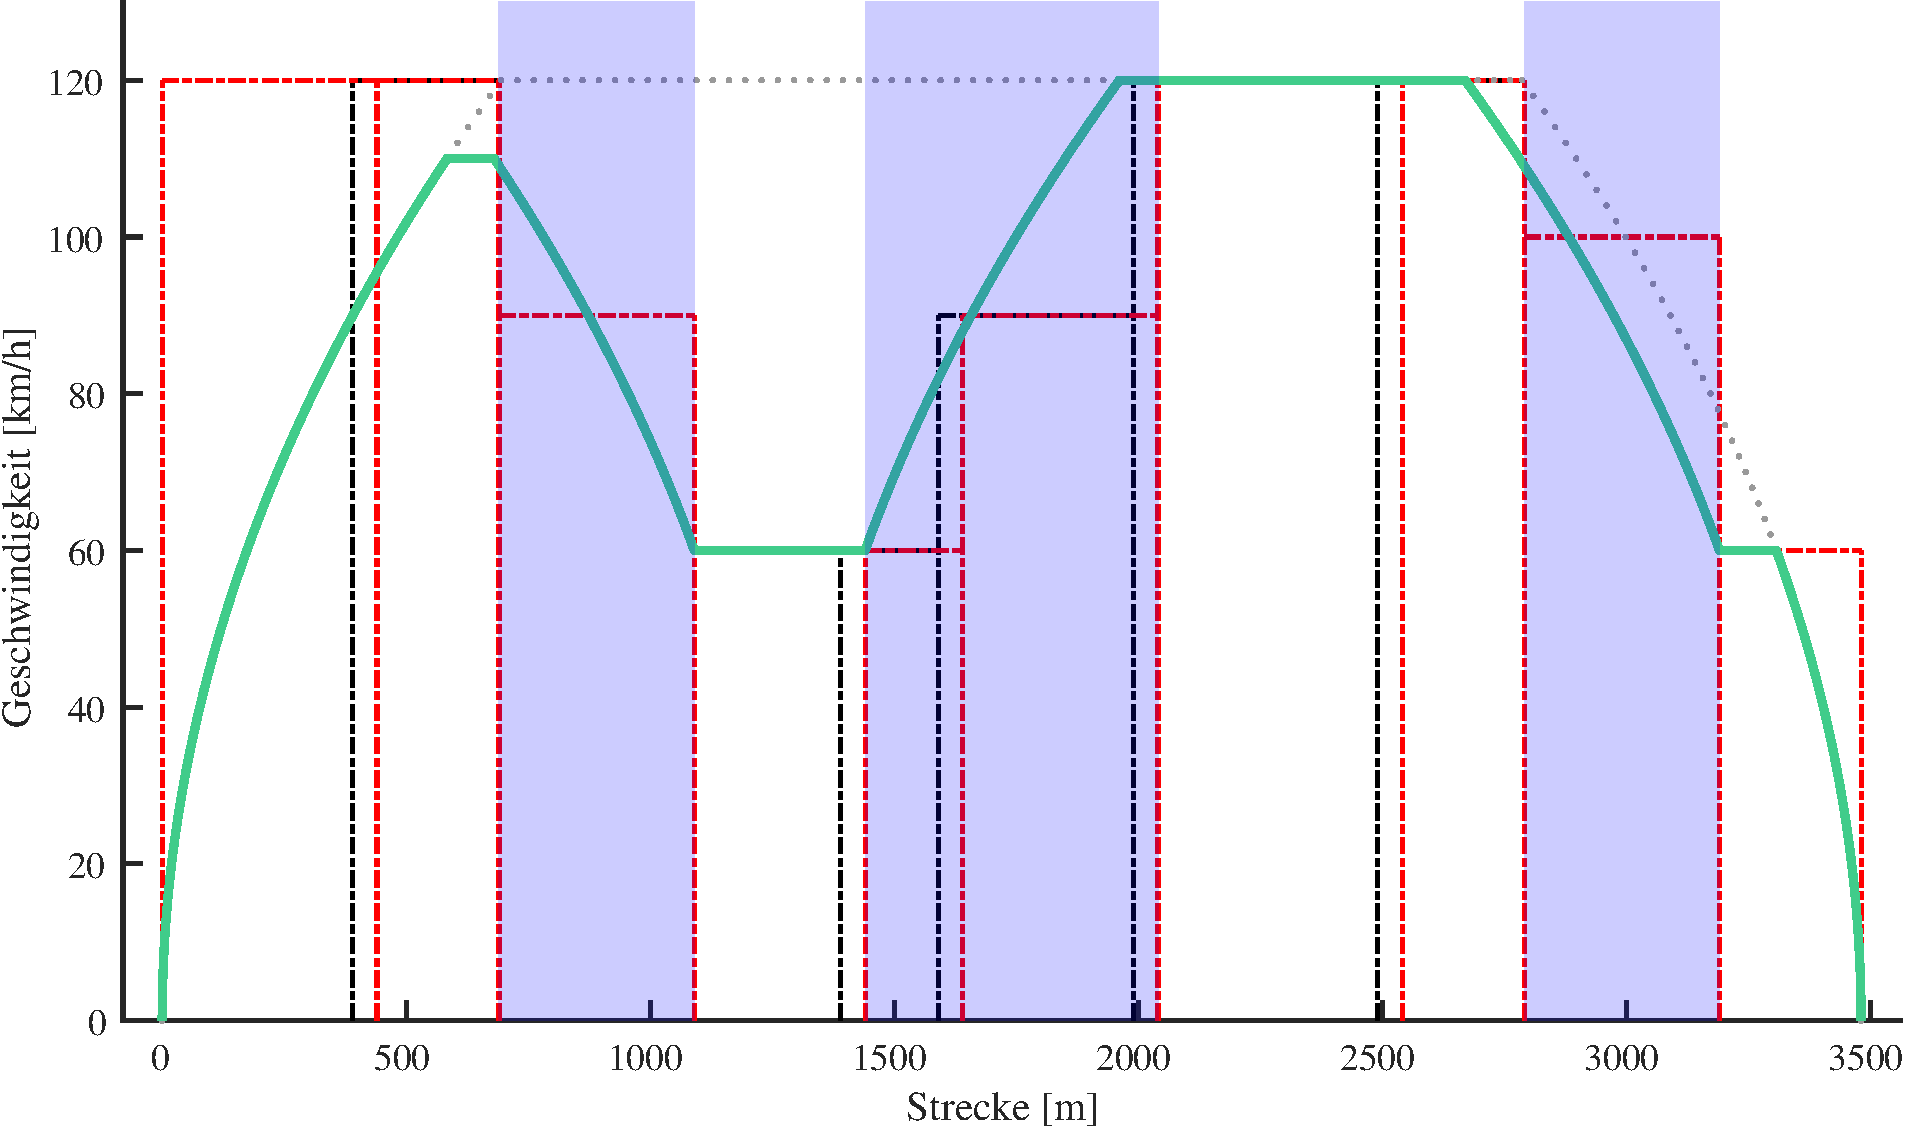
\includegraphics[width=\linewidth]{../images/matlab/it4.pdf}
\caption{Fahrtverlaufberechnung (2. Iteration)}
\label{fig:it4}
\end{figure}
\begin{figure}
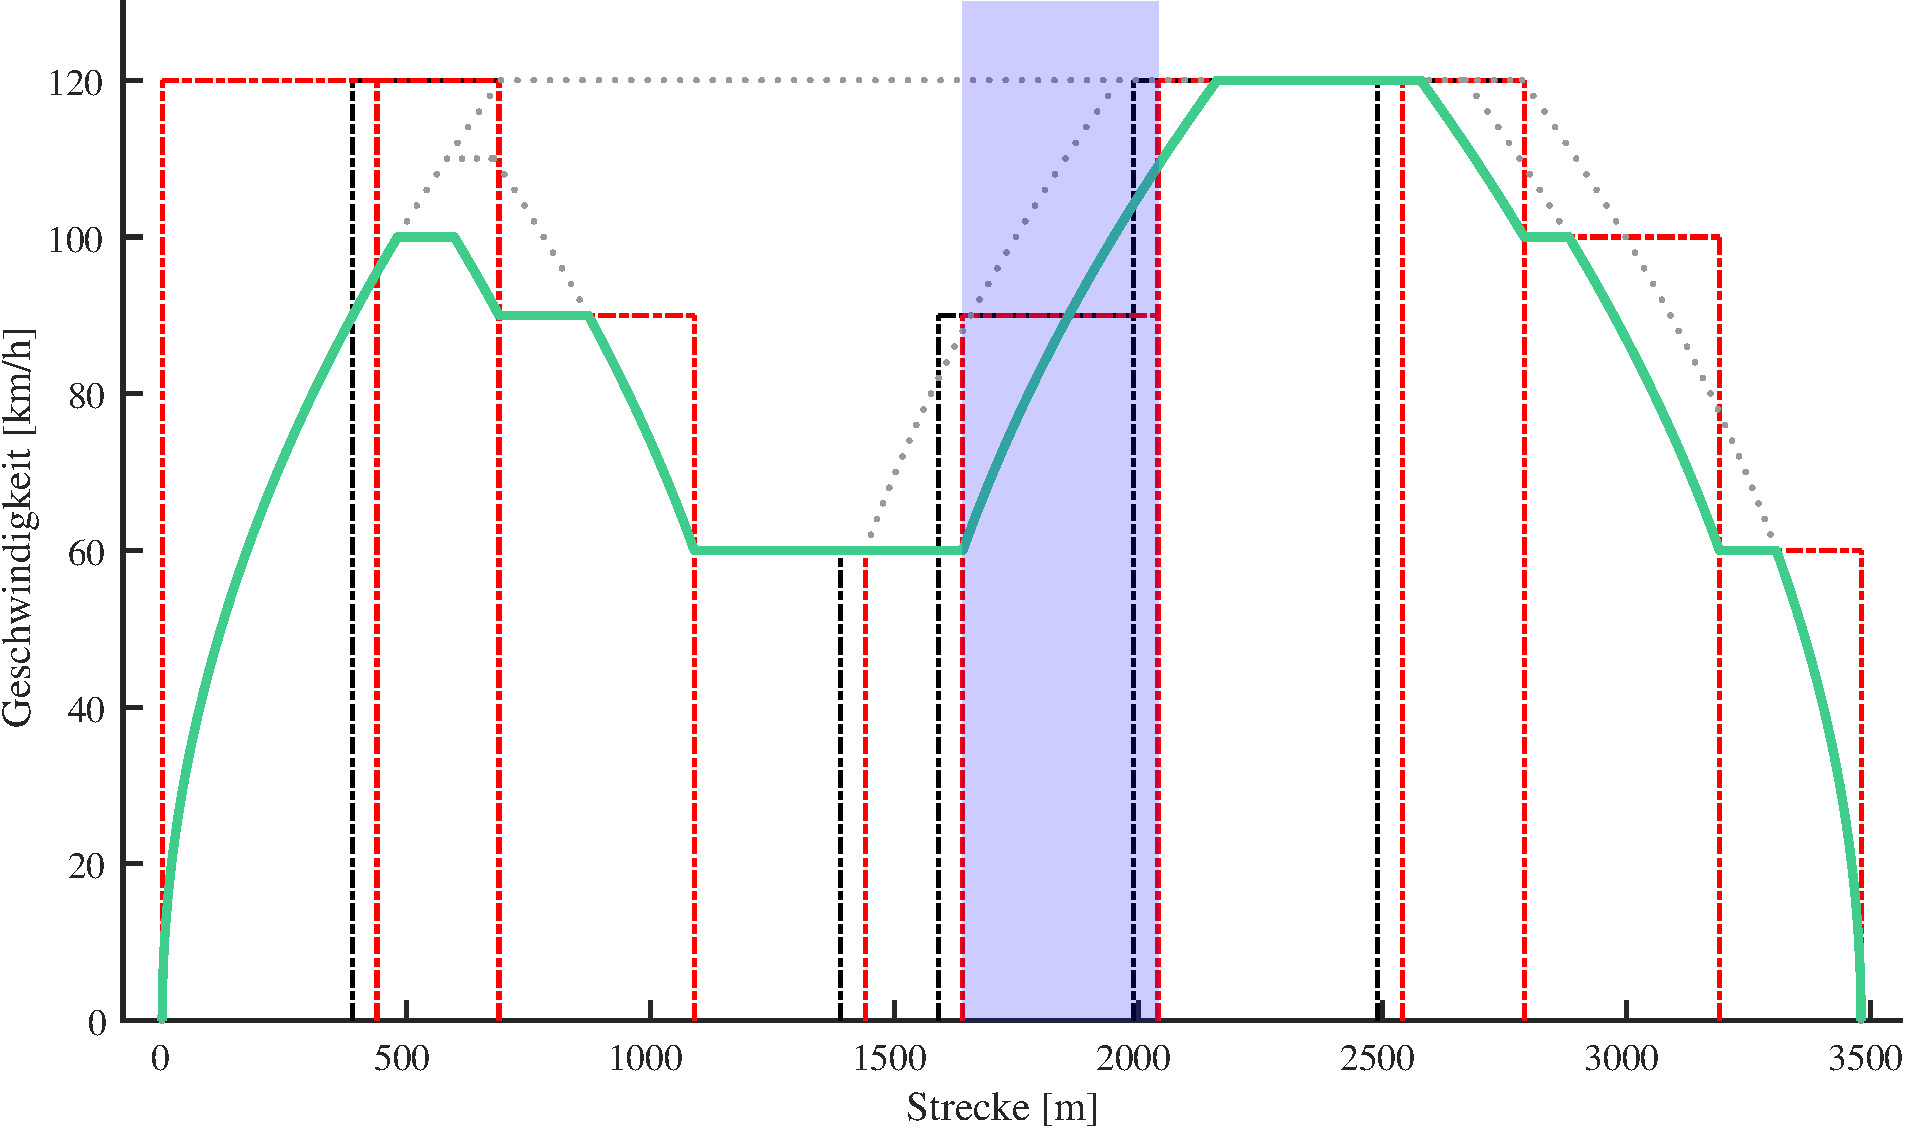
\includegraphics[width=\linewidth]{../images/matlab/it5.pdf}
\caption{Fahrtverlaufberechnung (3. Iteration)}
\label{fig:it5}
\end{figure}
\begin{figure}
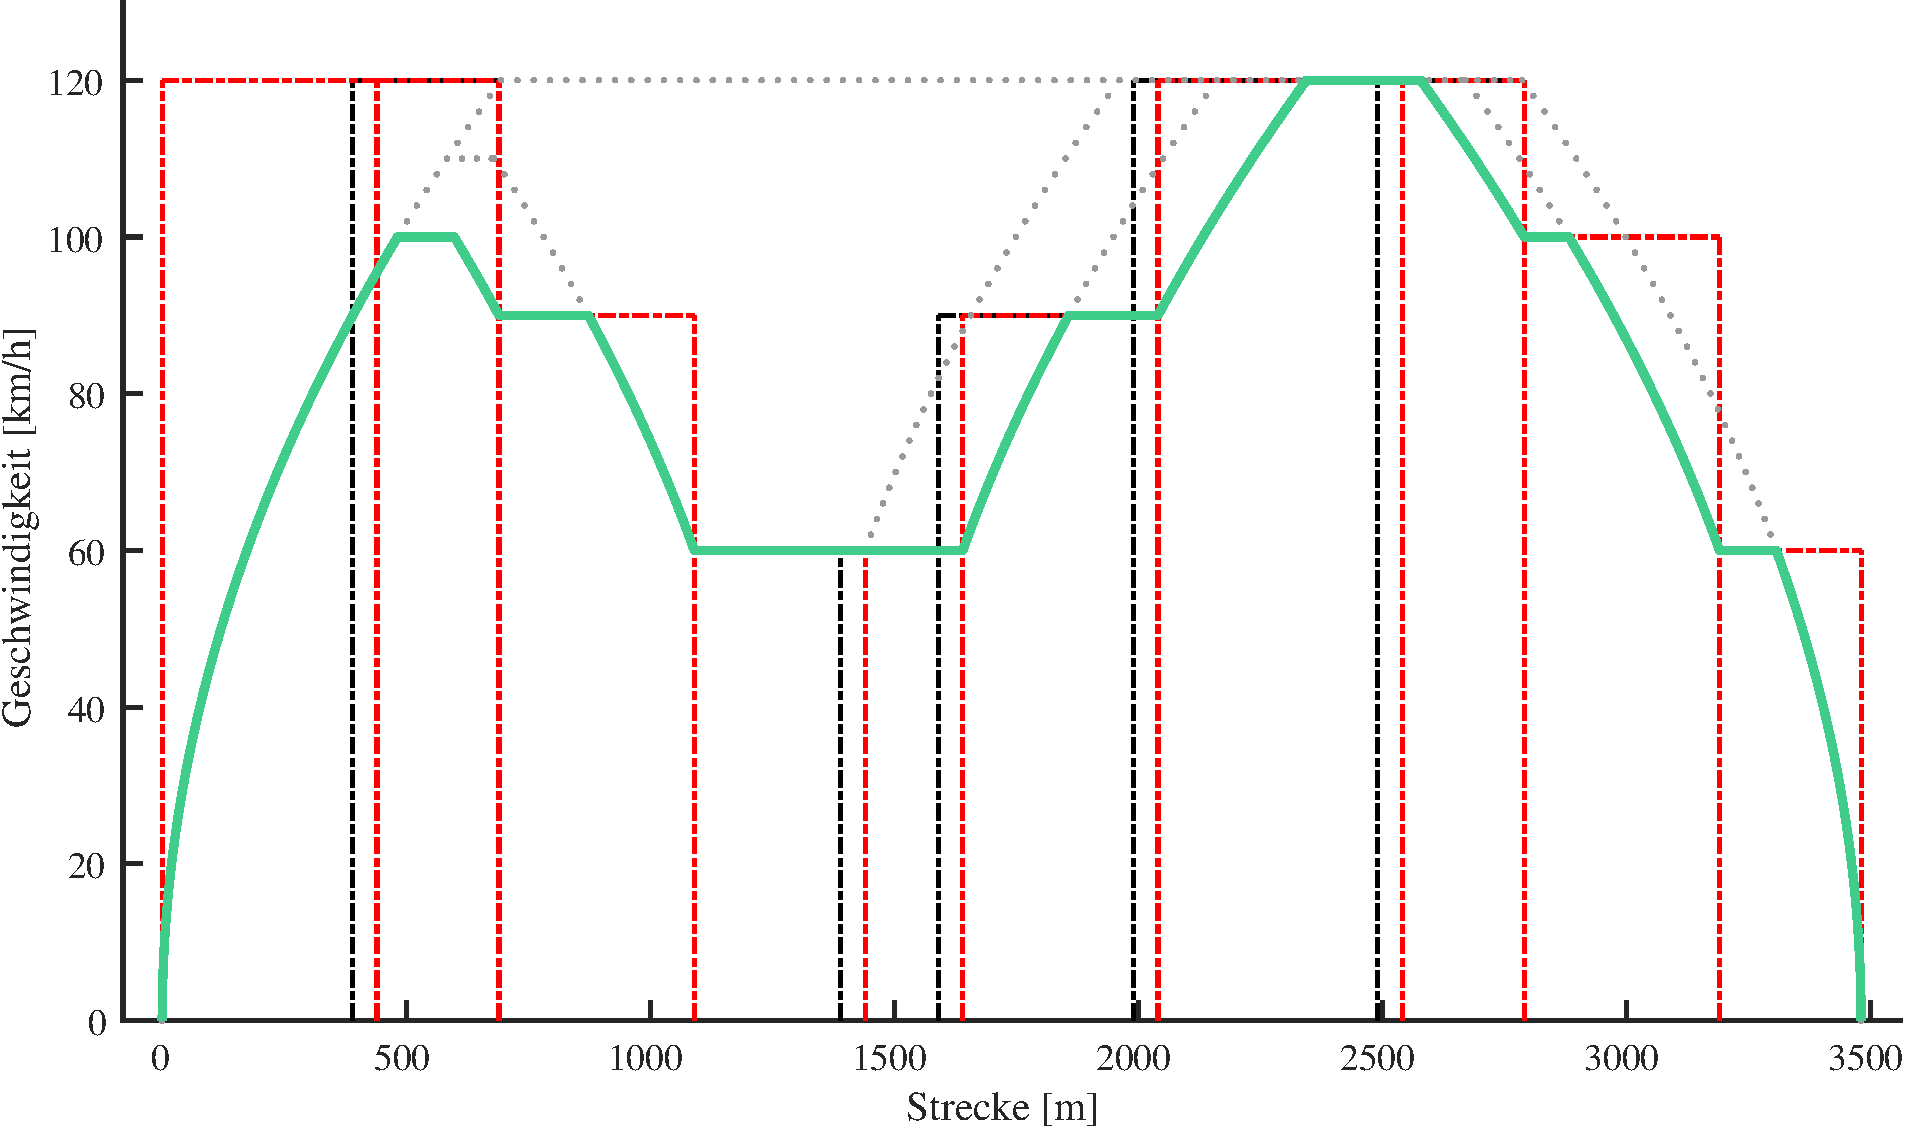
\includegraphics[width=\linewidth]{../images/matlab/it6.pdf}
\caption{Fahrtverlaufberechnung (4. Iteration)}
\label{fig:it6}
\end{figure}
\subsection{Einhaltung der Mindestzeit auf einer Geschwindigkeit} \label{minTime}
\begin{enumerate}
\item Ideal: möglichst späte v reduzieren
\end{enumerate}
Für eine möglichst realitätsnahe Simulation kann über die Variable \textit{\$globalTimeOnOneSpeed} in der Datei \textit{globalVariables.php} eine Mindestzeit festgelegt werden, die ein Fahrzeug auf einer Geschwindigkeit mindestens einhalten muss. Ebenfalls kann über die Variablen \textit{\$useMinTimeOnSpeed} und \textit{\$errorMinTimeOnSpeed} festgelegt werden, ob die Funktion aktiviert sein soll und ob es in dem Fall, dass diese Zeit nicht eingehalten werden kann, zu einer Fehlermeldung kommen soll. Im Falle einer Fehlermeldung würde das Fahrzeug nicht losfahren bzw. eine Gefahrenbremsung einleiten, falls das Fahrzeug aktuell eine Geschwindigkeit $v > 0$ hat. 
Wenn auf einem Abschnitt die Mindestzeit nicht eingehalten werden kann, kann eine Beschleunigung später eingeleitet werden, eine Verzögerung vorzeitiger eingeleitet werden oder auf eine kleinere Geschwindigkeit beschleunigt werden. In dem folgenden Algorithmus werden die \dots
Dadurch, dass sich eine Verschiebung einer Beschleunigung bzw. Verzögerung auf die nächsten Abschnitte auswirken kann, wird der \Gls{fahrtverlauf} in \textit{\$subsections} unterteilt. Eine \textit{\$subsection} beschreibt dabei den Bereich des \Gls{fahrtverlauf}s, in dem das Fahrzeug zum ersten Mal beschleunigt und zum letzten Mal abbremst. In der Darstellung \ref{fig:it7} wurde der exemplarische \Gls{fahrtverlauf} somit in zwei \textit{\$subsection} unterteilt, welche Lila bzw. Gelb hinterlegt sind.
\begin{figure}
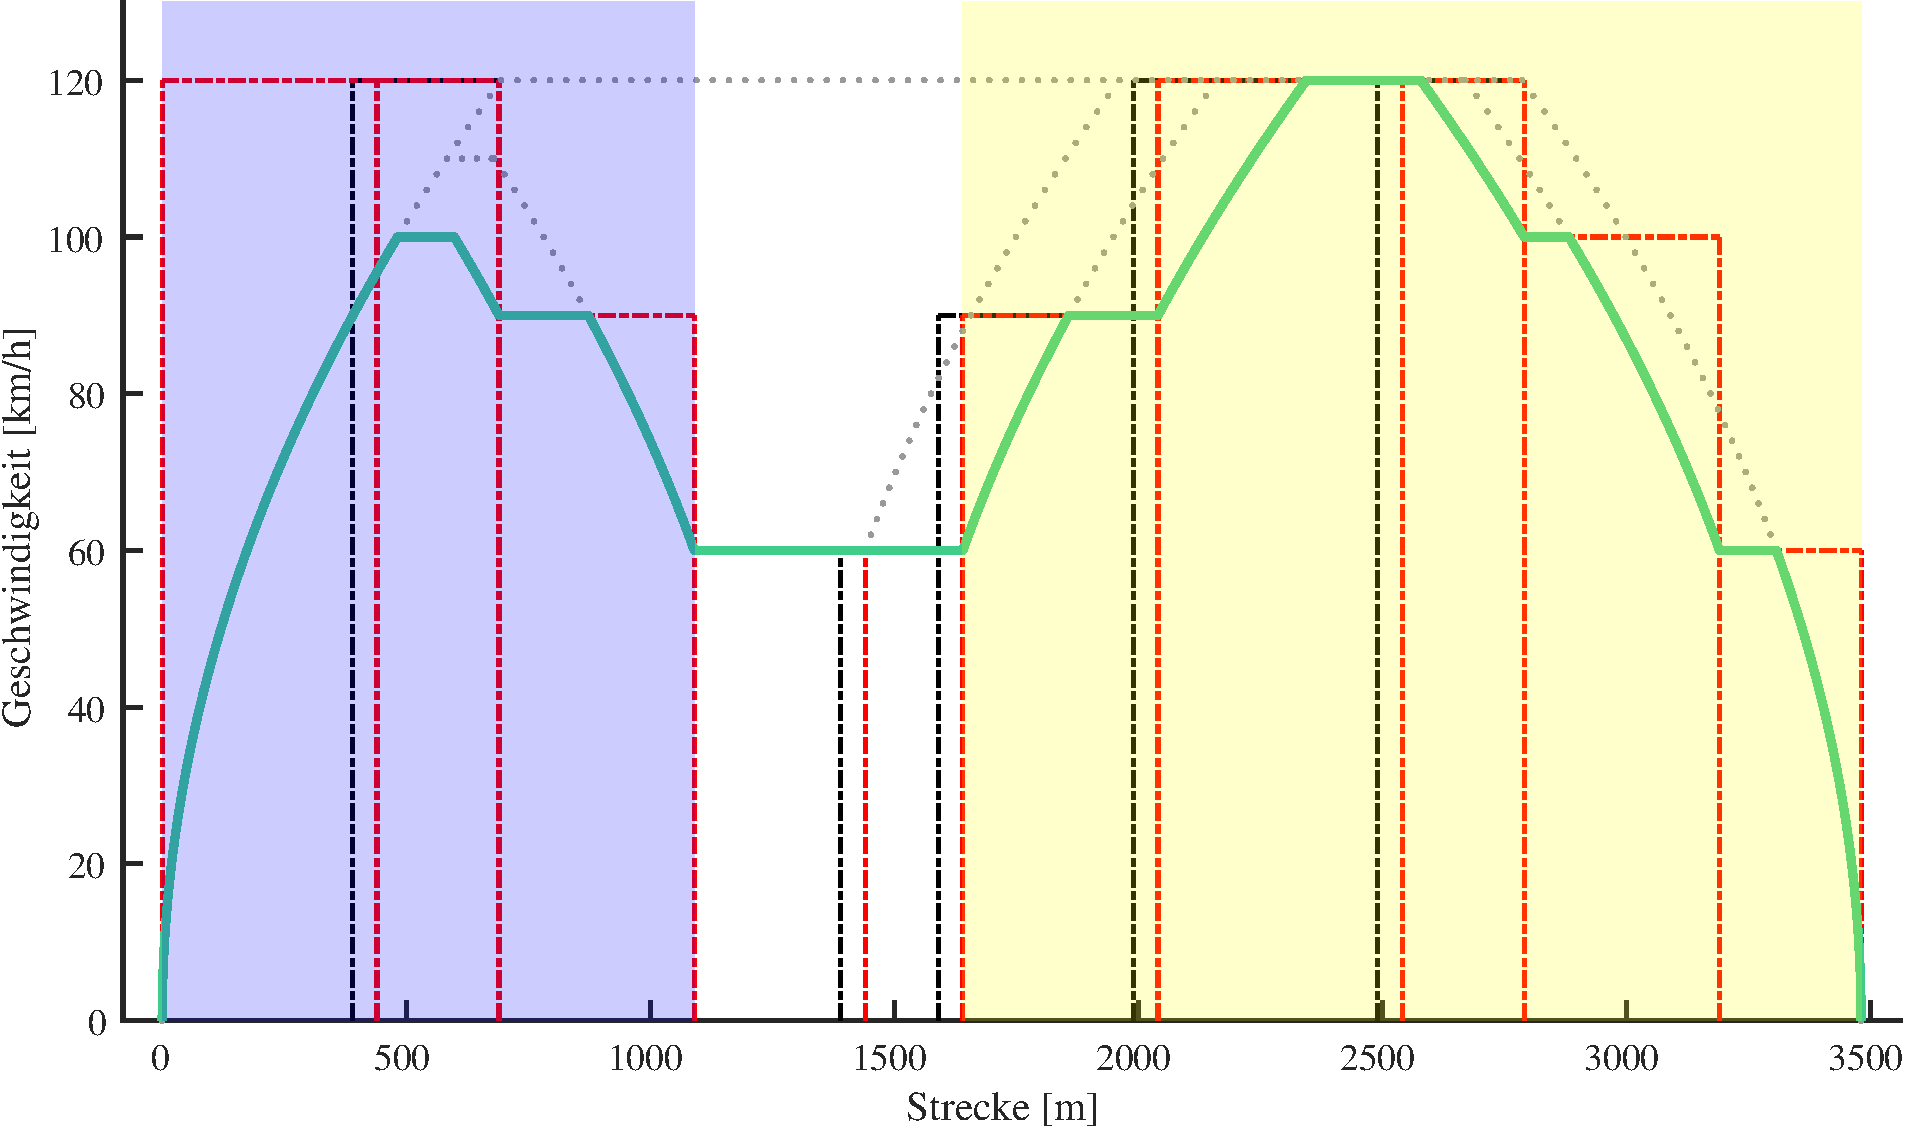
\includegraphics[width=\linewidth]{../images/matlab/it7.pdf}
\caption{Einteilung des \Gls{fahrtverlauf}s in \textit{\$subsections}}
\label{fig:it7}
\end{figure}
Diese Einteilung wird vorgenommen, da sich die Verschiebung einer Beschleunigung bzw. Verzögerung auf die folgenden bzw. vorherigen Abschnitte auswirkt. Durch diese Einteilung kann verhindert werden, dass es dadurch zu Konflikten kommt. Falls die Beschleunigungen bzw. Verzögerungen soweit nach hinten bzw. nach vorne verschoben werden müssen, kann die maximale Geschwindigkeit auf dieser \textit{\$subsection} reduziert werden und die zur Verfügung stehende Strecke vergrößert werden. Wie in Darstellung \ref{fig:it7} zu erkennen wird hierbei im ersten Schritt der Abschnitt zwischen zwei \textit{\$subsections} ausgelassen. Nach der Ermittlung der \textit{subsections} wird überprüft, ob auf den Abschnitten zwischen den \textit{\$subsections} die Mindestzeit eingehalten wird. Wenn das nicht der Fall ist, wird der Abschnitt automatisch dem in Fahrtrichtung hinteren \textit{\$subsection} zugeordnet. Dadurch wird sichergestellt, dass das Fahrzeug, wenn es an einer Stelle des \Gls{fahrtverlauf}s die Geschwindigkeit reduziert, dies möglichst spät tut.
Nachdem die \textit{\$subsections} mittels der Funktion \textit{createSubsections$($$)$} erstellt wurden und mit der Funktion \textit{array\_reverse$($$)$} in umgekerte Reihenfolge in dem Array \textit{\$subsection\_list} gesammelt wurden, wird für jede \textit{\$subsection} überprüft, ob die Beschleunigungen bzw. Verzögerungen verschoben werden können. Dabei wird über alle konstanten Geschwindigkeiten iteriert, überprüft, ob die Mindestzeit eingehalten wird und wenn das nicht der Fall ist, wird überprüft, ob eine Verschiebung möglich ist. Sollte bei einer Verschiebung die $position\_1$ des \textit{\$keyPoints} hinter $position\_0$ des zweiten \textit{\$keyPoints} liegen (bei einer Beschleunigung), wird der zweite \textit{\$keyPoint} gelöscht. Gleiches geschieht bei der Verzögerung in umgekehrter Reihenfolge. Nach der Verschiebung wird überprüft, ob auf allen konstanten Geschwindigkeit die Mindestzeit eingehalten wird. Wenn das der Fall ist, wird die nächste \textit{\$subsection} überprüft. In dem Fall, dass durch die Verschiebung die Mindestzeit nicht eingehalten werden kann, wird die maximale Geschwindigkeit auf dieser \textit{\$subsection} um $10 km/h$ reduziert, die \textit{\$subsections} neu berechnet und erneut über alle \textit{\$subsection} iteriert. Die Neuberechnung ist notwendig, da durch die Reduzierung der Geschwindigkeit die \textit{\$subsections} anders aufgeteilt sein können.
Wenn alle \textit{\$subsections} die Mindestzeit einhalten, wird der Algorithmus beendet. In der Darstellung \ref{fig:it9} ist der \Gls{fahrtverlauf} unter Einhaltung der Mindestzeit auf einer Geschwindigkeit abgebildet.
\begin{figure}
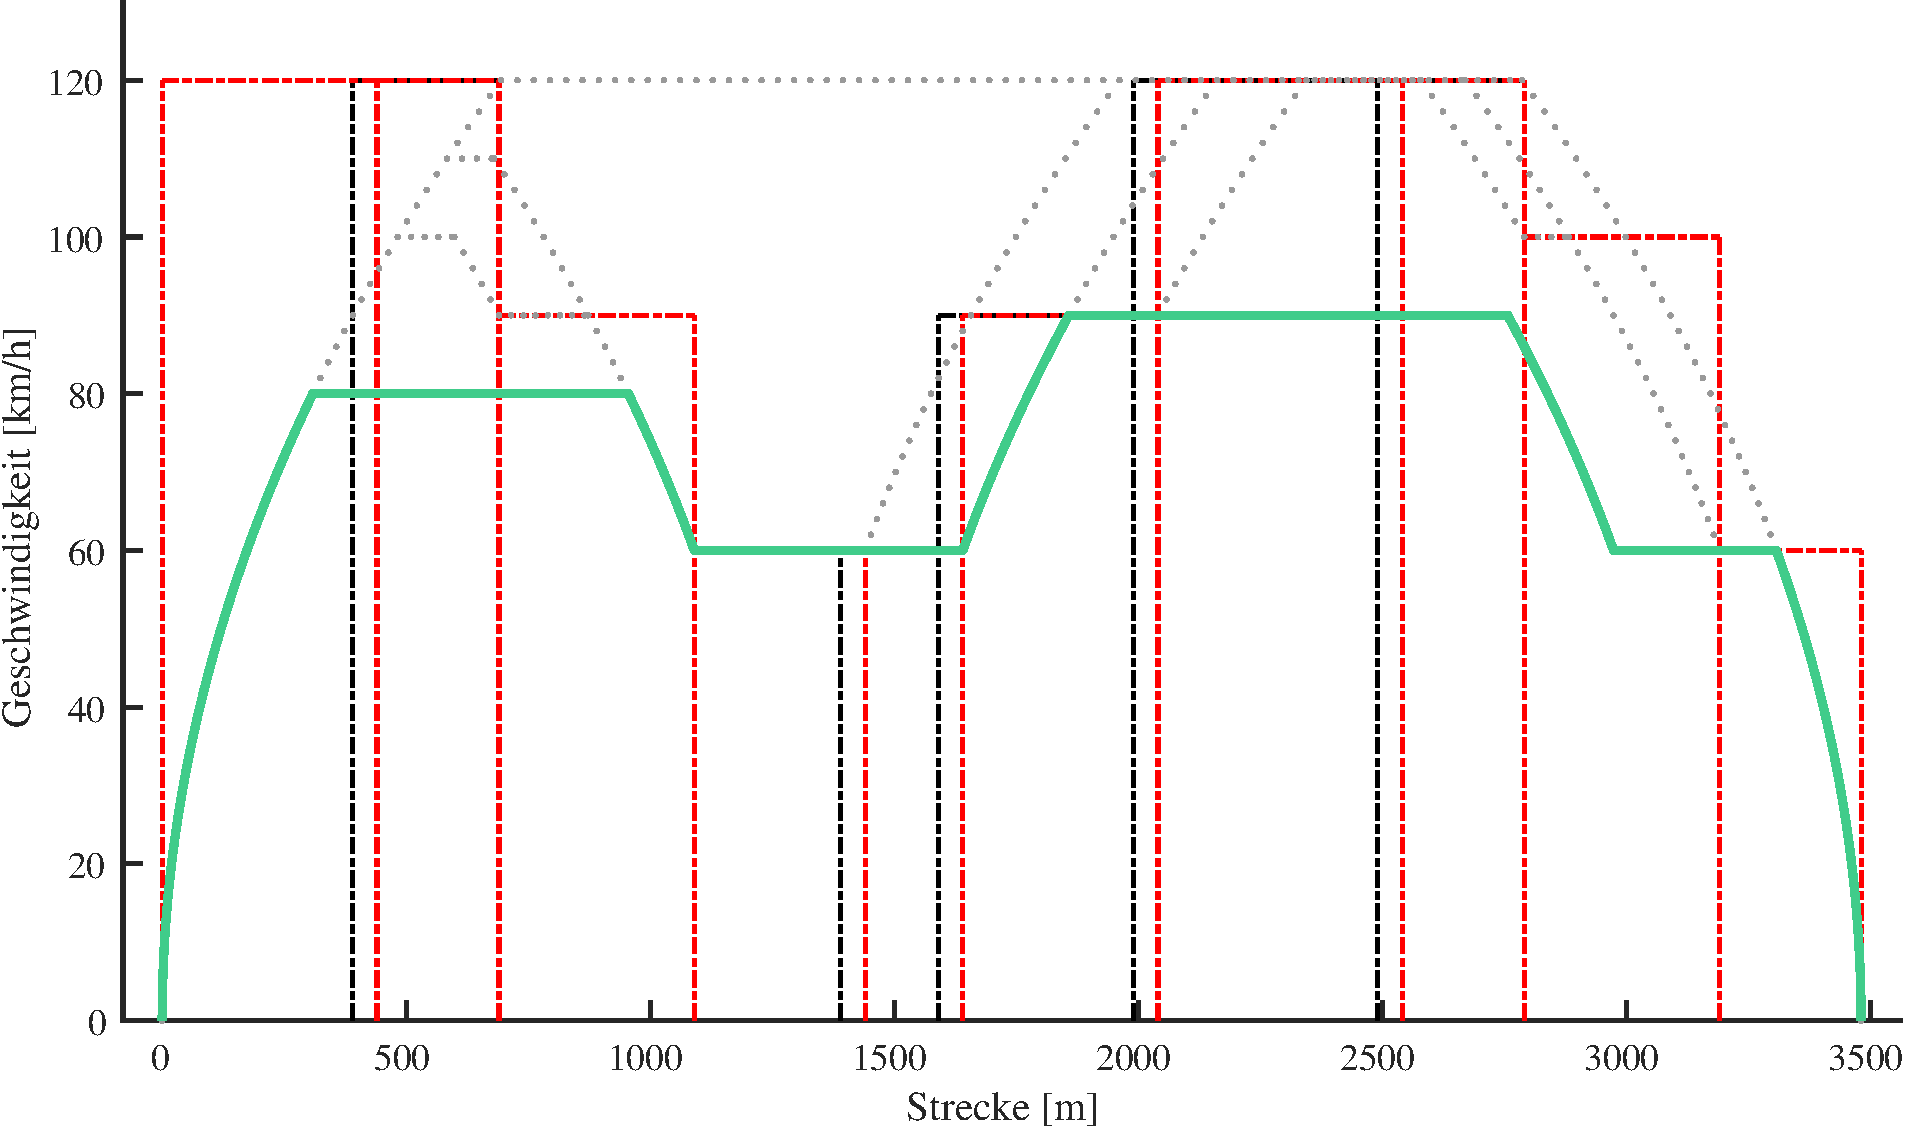
\includegraphics[width=\linewidth]{../images/matlab/it9.pdf}
\caption{Fahrtverlauf unter Einhaltung der Mindestzeit}
\label{fig:it9}
\end{figure}
\begin{table}
\begin{center}
\renewcommand{\arraystretch}{1.2}
\begin{tabular}{c|c}
Index & Funktion \\ \hline
\textit{max\_index}                 	&  	\makecell{ndex des \textit{\$keyPoints} mit der Beschleunigung auf die\\maximale Geschwindigkeit in der \textit{\$subsection}}     \\ \hline
\textit{indexes}                 		&    	Indexe aller beinhalteten \textit{\$keyPoints}                  \\ \hline
\textit{is\_prev\_section}           	&   	Berücksichtigung des Abschnitts vor der \textit{\$subsection}     \\ \hline
\textit{is\_next\_section}           	&     	Berücksichtigung des Abschnitts nach der \textit{\$subsection}                 \\ \hline
\textit{failed}                 		&   	Unterschreitung der Mindestzeit auf der \textit{\$subsection}     \\ 
\end{tabular}
\renewcommand{\arraystretch}{1}
\caption{Aufbau des \textit{\$subsection}-Arrays}
\label{table:subsection}
\end{center}
\end{table}
Für den Fall, dass das Fahrzeug auf einer Geschwindigkeit die Mindestzeit nicht einhält und als nächstes beschleunigen würde, kann die Beschleunigung später eingeleitet werden. 
\subsection{Berücksichtigung der Ankunftszeit bei der Berechnung des \Gls{fahrtverlauf}s} \label{time}
Der berechnete \Gls{fahrtverlauf} in den Kapiteln \ref{v_max}, \ref{überprüfung}, \ref{neuberechnung} und \ref{minTime} ermittelt die frühstmögliche Ankunftszeit am Ziel. In dem Fall, dass der Zug dadurch mit einer Verspätung am Ziel ankommt wird der \Gls{fahrtverlauf} an das Fahrzeug übergeben. Falls der Zug allerdings mit dem \Gls{fahrtverlauf} zu früh am Ziel ankommen würde, wird überprüft, ob es möglich ist die Geschwindigkeit zu reduzieren, sodass der Zug energieeffizienter fahren kann und ohne Verspätung am Ziel ankommt.
Ergebnis ist in \ref{fig:it9} abgebildet.
Im ersten Schritt wird mittels der Funktion \textit{checkIfTheSpeedCanBeDecreased$($$)$} überprüft, ob die Geschwindigkeit reduziert werden kann. Dabei werden alle \textit{\$keyPoints} ermittelt, bei denen das Fahrzeug beschleunigt und die beim darauffolgenden \textit{\$keyPoint} abbremsen. Für jeden dieser \textit{\$keyPoints} werden die möglichen Geschwindigkeiten ermittelt, welche das Fahrzeug zwischen den beiden \textit{\$keyPoints} fahren könnte. Für die Berechnung dieser Geschwindigkeiten wird als niedrigste Geschwindigkeit die \textit{speed\_0} des ersten \textit{\$keyPoints} bzw. \textit{speed\_1} des zweiten \textit{\$keyPoints} - jenachdem, welche niedriger ist - genommen und in 10 $km/h$-Schritten bis  \textit{speed\_1} des ersten \textit{\$keyPoints} abgespeichert. Daraus ergibt sich für jeden \textit|{\$keyPoint} eine \textit{range} an möglichen Geschwindigkeiten. Als Rückgabewert der Funktion wird ein \textit{Array} wiedergegeben, welches die Einträge \textit{possible} und \textit{range} enthält und als \textit{\$returnSpeedDecrease} abgespeichert. Der Eintrag \textit{possible} gibt an, ob das Fahrzeug auf dem gesamten \Gls{fahrtverlauf} die Geschwindigkeit reduzieren könnte und wird als Boolescher Wert (\textit{true}/\textit{false}) abgespeichert und und in dem \textit{Array} \textit{range} werden alle Indexe der möglichen \textit{\$keyPoints} inklusive der ermittelten Geschwindigkeiten abgespeichert.
In dem in Abbildung \ref{fig:it9} dargestellten \Gls{fahrtverlauf} wären so für den \textit{\$keyPoint} mit dem Index 0 (die Indexe der \textit{\$keyPoints} entsprechen dem Zahlenbereich der $\mathbb{N}_0$) die Geschwindigkeiten 60, 70 und 80 $km/h$ ermittelt worden und für den \textit{\$keyPoint} mit dem Index $2$ die Geschwindigkeiten 60, 70, 80 und 90 $km/h$.
Wenn eine Reduzierung der Geschwindigkeit möglich ist, wird in einer \textit{while}-Schleife versucht die Geschwindigkeit zu reduzieren, bis das Fahrzeug bei der nächsten Reduzierung mit einer Verspätung am Ziel ankommen würde oder eine weitere Reduzierung nicht möglich ist, da die Maximalgeschwindigkeit auf dem \Gls{fahrtverlauf} 10 $km/h$ beträgt. Innerhalb der \textit{while}-Schleife ermittelt die Funktion \textit{findMaxSpeed$($$)$} aus dem \textit{\$returnSpeedDecrease}-Array den \textit{\$keyPoint} mit der höchsten Geschwindigkeit. Für den Fall, dass mehrere \textit{\$keyPoints} die selbe Höchstgeschwindigkeit haben, wird der letzte dieser \textit{\$keyPoints} ermittelt. Im Anschluss wird mit einer \textit{for}-Schleife in 10er-Schritten in absteigender Reihenfolge über die möglichen Geschwindigkeiten iteriert und überprüft, ob durch die Anpassung die Ankunftszeit eingehalten werden kann. Sobald die Ankunftszeit nicht eingehalten werden kann, werden die \textit{\$keyPoints} aus dem vorherigen Iterationsschritt gespeichert und die \textit{while}-Schleife wird abgebrochen. Sollte die \textit{for}-Schleife durchlaufen, ohne dass es zu einer Überschreitung der maximal verfügbaren Zeit kommt, wird die Funktion \textit{checkIfTheSpeedCanBeDecreased$($$)$} erneut aufgerufen. 
Das Ergebnis dieser Berechnung ist in der Abbildung \ref{fig:it10} zu sehen.
\begin{figure}
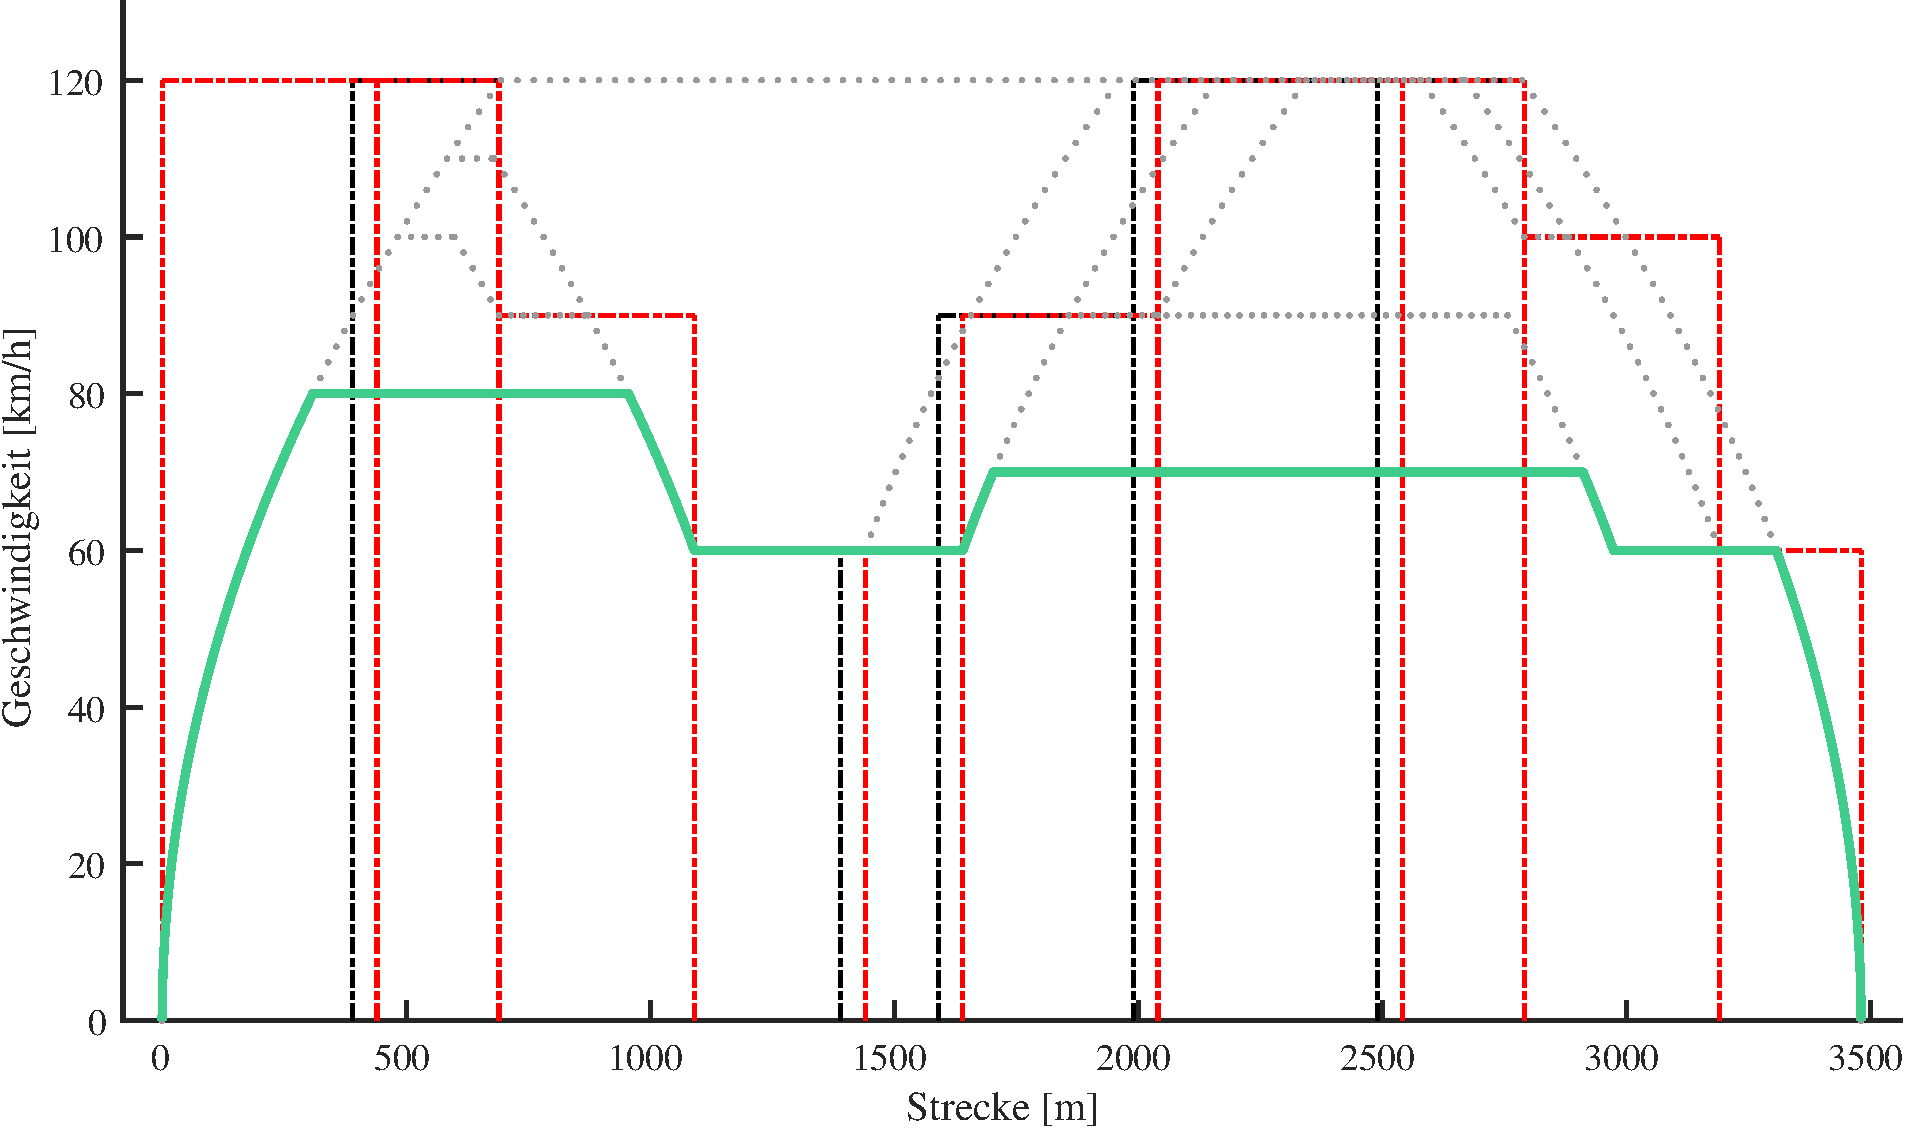
\includegraphics[width=\linewidth]{../images/matlab/it10.pdf}
\caption{\Gls{fahrtverlauf} mit reduzierter Geschwindigkeit unter Einhaltung der Ankunftszeit}
\label{fig:it10}
\end{figure}
\subsection{Berücksichtigung der exakten Ankunftszeit bei der Berechnung des \Gls{fahrtverlauf}s} \label{time2}
Die in Kapitel \ref{minTime} errechnete Ankunftszeit, beschreibt die spätmöglichste Ankunftszeit am Ziel, ohne dass das Fahrzeug mit einer Verspätung am Ziel ankommt, wenn bei einer Beschleunigung auf eine geringere Zielgeschwindigkeit beschleunigt wird. Dadurch wird das Fahrzeug im Normalfall noch nicht exakt pünktlich das Ziel erreichen. Über die Variable \textit{\$useSpeedFineTuning} kann festgelegt werden, ob das Fahrzeug eine exakte Ankunftszeit versuchen soll zu erreichen. Wenn diese Funktion aktiviert ist und der Eintrag \textit{possible} aus dem Array \textit{\$returnSpeedDecrease} \textit{true} ist, wird für den letzten \textit{\$keyPoint} aus dem \textit{\$returnSpeedDecrease}-Array überprüft, ob die Verzögerung des nächsten \textit{\$keyPoints} vorzeitiger eingeleitet werden kann. Sollte die Zielgeschwindigkeit der Verzögerung 0 $km/h$ sein, wird die Verzögerung unterteilt in eine Verzögerung auf 10 $km/h$ und eine von 10 $km/h$ auf 0 $km/h$. Die Position der vorzeitig eingeleiteten Verzögerung wird mittels der Funktion \textit{speedFineTuning$($$)$} berechnet, welche als Parameter den Betrag der Differenz zwischen aktueller Soll- und Ist-Ankunftszeit und den Index des vorherigen \textit{\$keyPoints} übergeben bekommt.
\begin{figure}
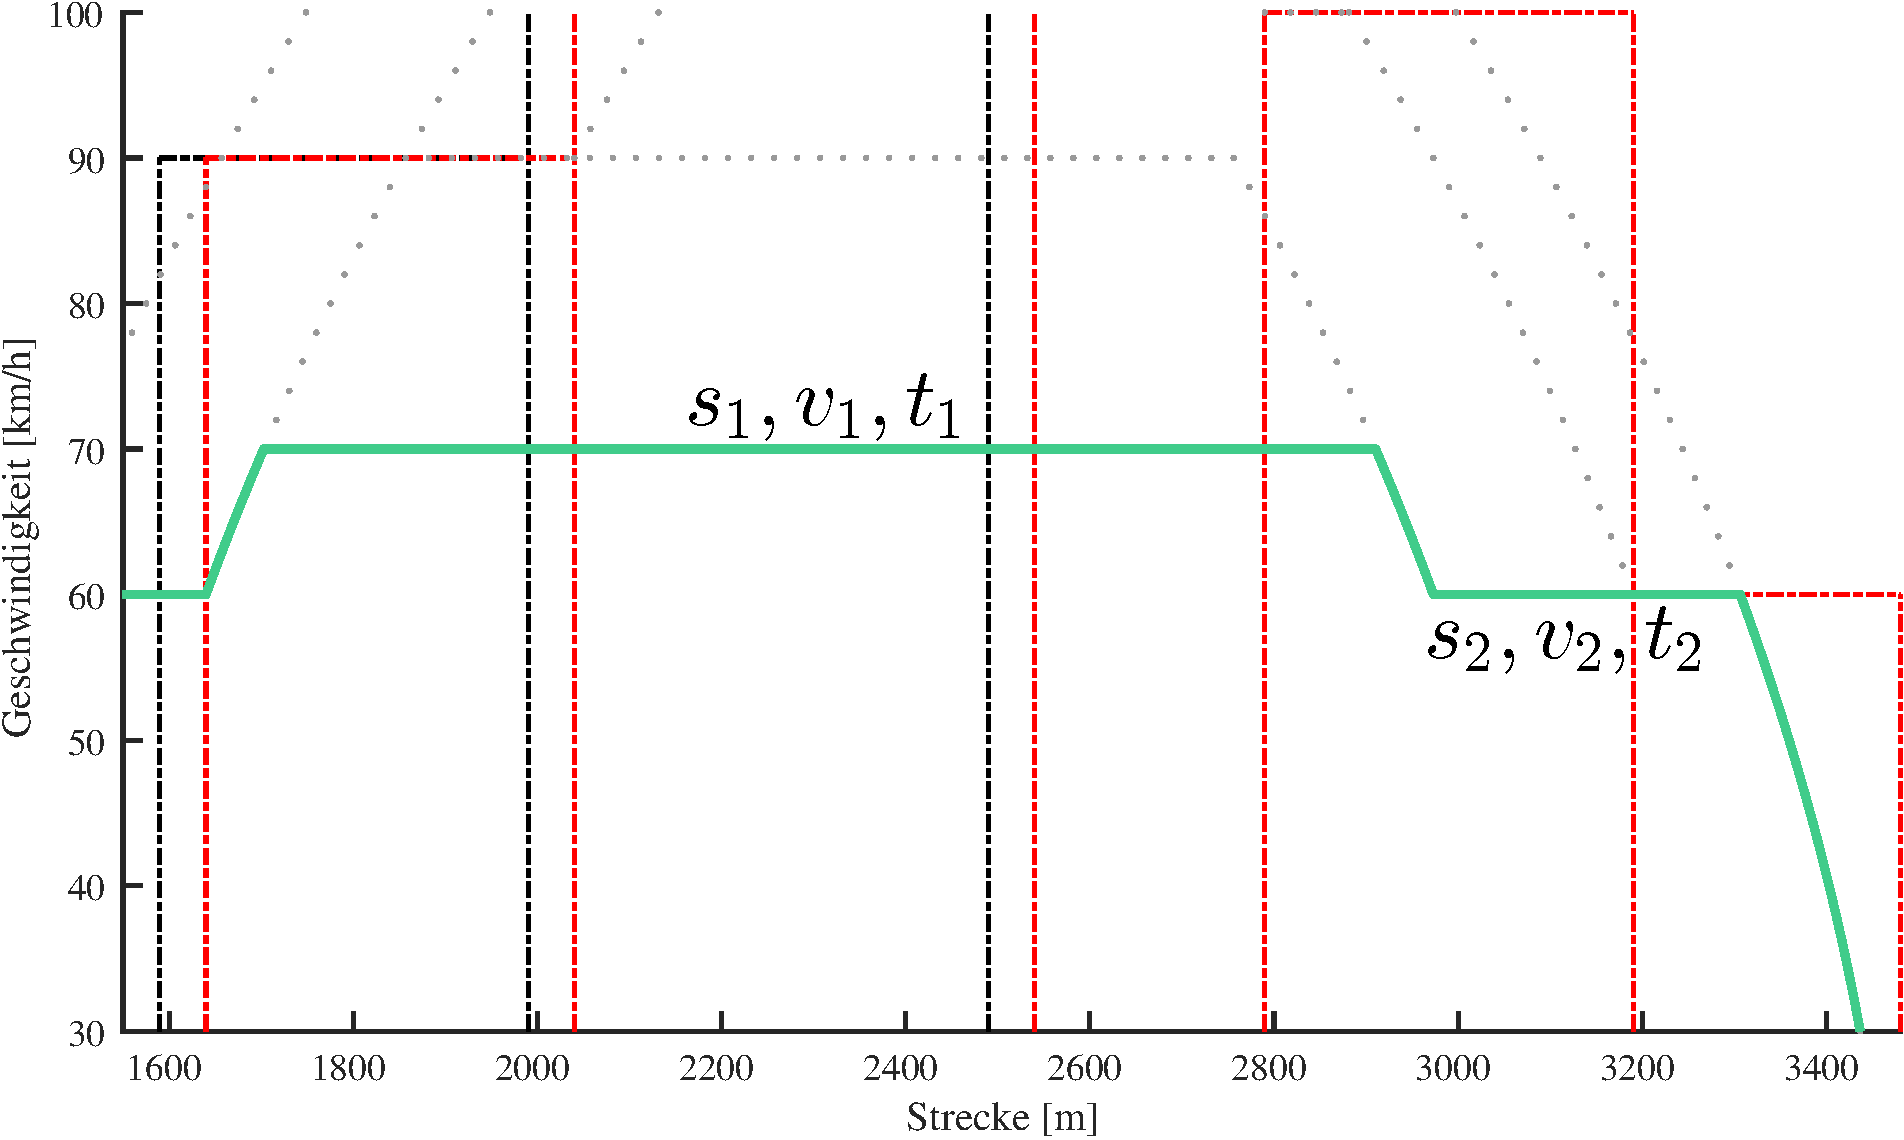
\includegraphics[width=\linewidth]{../images/matlab/it11.pdf}
\caption{speedFineTuning\_1}
\label{fig:it11}
\end{figure}
In Abbildung \ref{fig:it11} werden die Geschwindigkeiten ($v_1$,$v_2$), Strecken ($s_1$,$s_2$) und Zeiten ($t_1$,$t_2$) vor und nach der Verzögerung, welche vorzeitiger eingeleitet werden soll, um eine pünktliche Ankunft am Ziel zu ermöglichen, dargestellt und in Tabelle \ref{table:speed_fine_tuning_ex} sind die exakten Werte des exemplarischen \Gls{fahrtverlauf}s aufgelistet, damit die verwendete Gleichung (Gleichung \ref{eq:t_1_tuning} aus Kapitel \ref{formula}) an diesem Beispiel angewandt werden kann. In diesem konkreten Beispiel würde das Fahrzeug 3,31 $s$ ($t_{\varDelta}$) zu früh an der Haltestelle ankommen, wodurch das Fahrzeug für die Zurücklegung der Strecken $s_1$ und $s_2$ insgesamt 85,42$s$ ($t_{ges}=t_1+t_2+t_{\varDelta}$) zur Verfügung hat.
\begin{table}
\begin{center}
\renewcommand{\arraystretch}{1.2}
\begin{tabular}{r L{3cm}}
$v_1$                   &   70 $km/h$ (19,44$m/s$)                         \\ 
$v_2$                   &   60 $km/h$ (16,67$m/s$)                         \\ 
$s_1$                   &   1207,67 $m$                         \\ 
$s_2$                   &   333,33 $m$                         \\ 
$s_{ges}$                   &   1541 $m$                         \\ 
$t_1$                   &   62,11 $s$                         \\ 
$t_2$                   &   20 $s$                         \\ 
$t_{\varDelta}$                   &   3,31 $s$                         \\ 
$t_{ges}$                   &   85,42 $s$                         \\ 
\end{tabular}
\renewcommand{\arraystretch}{1}
\caption{Geschwindigkeiten, Strecken und Zeiten vor und nach der Verzögerung}
\label{table:speed_fine_tuning_ex}
\end{center}
\end{table}
Durch das Einsetzen dieser Werte in die Gleichung \ref{eq:t_1_tuning} aus dem Kapitel \ref{formula} ergibt sich für $t_3$ ($t_3$, $t_4$, $s_3$ und $s_4$ bezeichnen die Strecken und Zeiten nach der Anpassung) ein Wert von 42,2$s$. Dementsprechend muss die Verzögerung 19,85$s$ ($t_1$ - $t_3$) früher eingeleitet werden
\begin{figure}
\[t_{3} = \frac{1541m - 16,67 m/s \cdot 85,42 s}{19,44 m/s - 16,67 m/s}\]
%\[t_{3} = \frac{1541m - 1423,95 m}{2,77 m/s}\]
%\[t_{3} = \frac{117,05 m}{2,77 m/s}\]
\[t_{3} = 42,26 s\]
\end{figure}
Die vorzeitige Einleitung der Verzögerung sorgt dafür, dass das Fahrzeug seinen nächsten Haltepunkt genau pünktlich erreicht und ist in Abbildung \ref{fig:it12} dargestellt, wobei durch die gepunktete Linie der \Gls{fahrtverlauf} vor der Anpassung zu sehen ist. Die neu berechneten Werte sind in Tabelle \ref{table:speed_fine_tuning_ex_2} aufgelistet.
\begin{figure}
  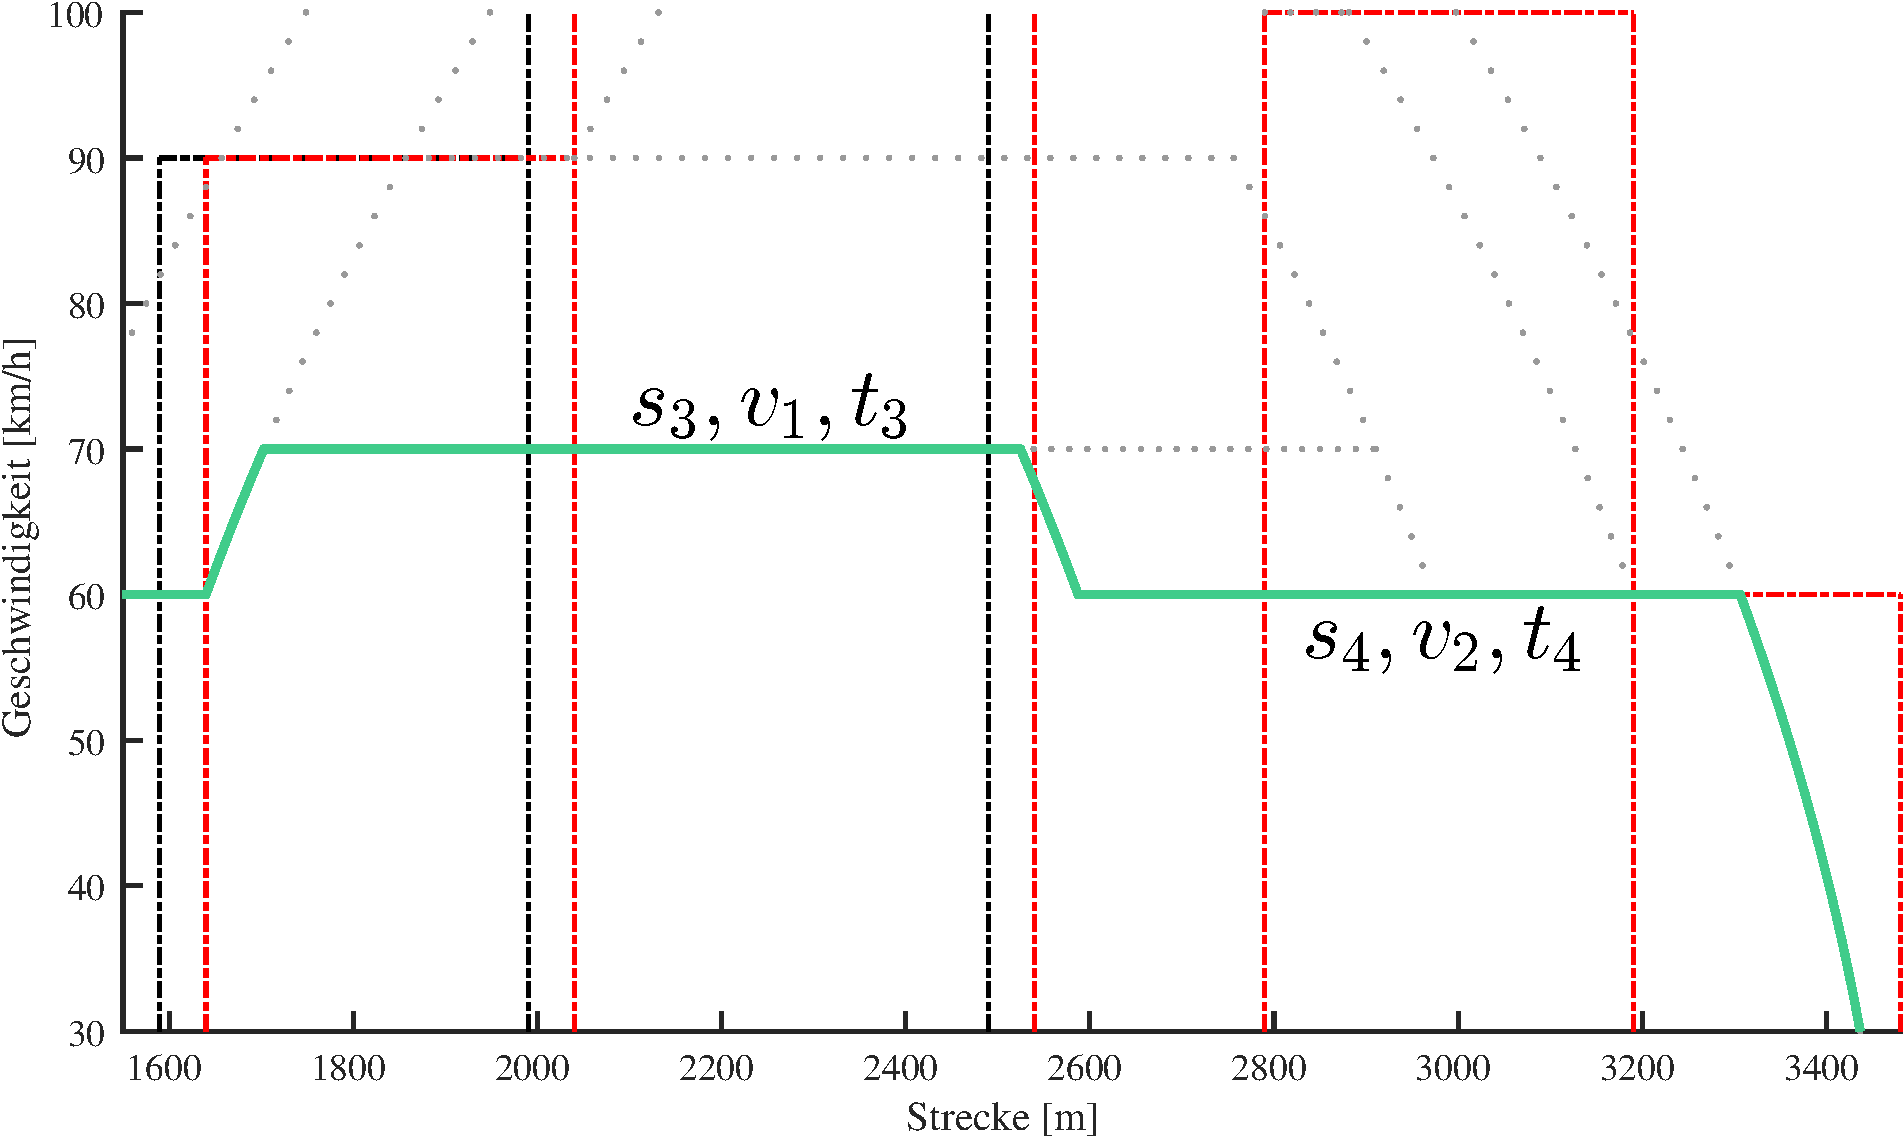
\includegraphics[width=\linewidth]{../images/matlab/it12.pdf}
  \caption{speedFineTuning\_2}
  \label{fig:it12}
\end{figure}
\begin{table}
\begin{center}
\renewcommand{\arraystretch}{1.2}
\begin{tabular}{r L{3cm}}
$s_3$                   	&   821,91$m$                      	\\ 
$s_4$                   	&   719,1$m$                         	\\ 
$t_3$                   	&   42,26$s$                         	\\ 
$t_4$                   	&   43,16$s$                         	\\ 
%$t_{ges}$           	&   85,42 $s$                         	\\ 
\end{tabular}
\renewcommand{\arraystretch}{1}
\caption{Geschwindigkeiten, Strecken und Zeiten vor und nach der Verzögerung nach der Anpassung}
\label{table:speed_fine_tuning_ex_2}
\end{center}
\end{table}
Der finale \Gls{fahrtverlauf} ist in Abbildung \ref{fig:it13} dargestellt und kann so dem Fahrzeug übergeben werden.
\begin{figure}
  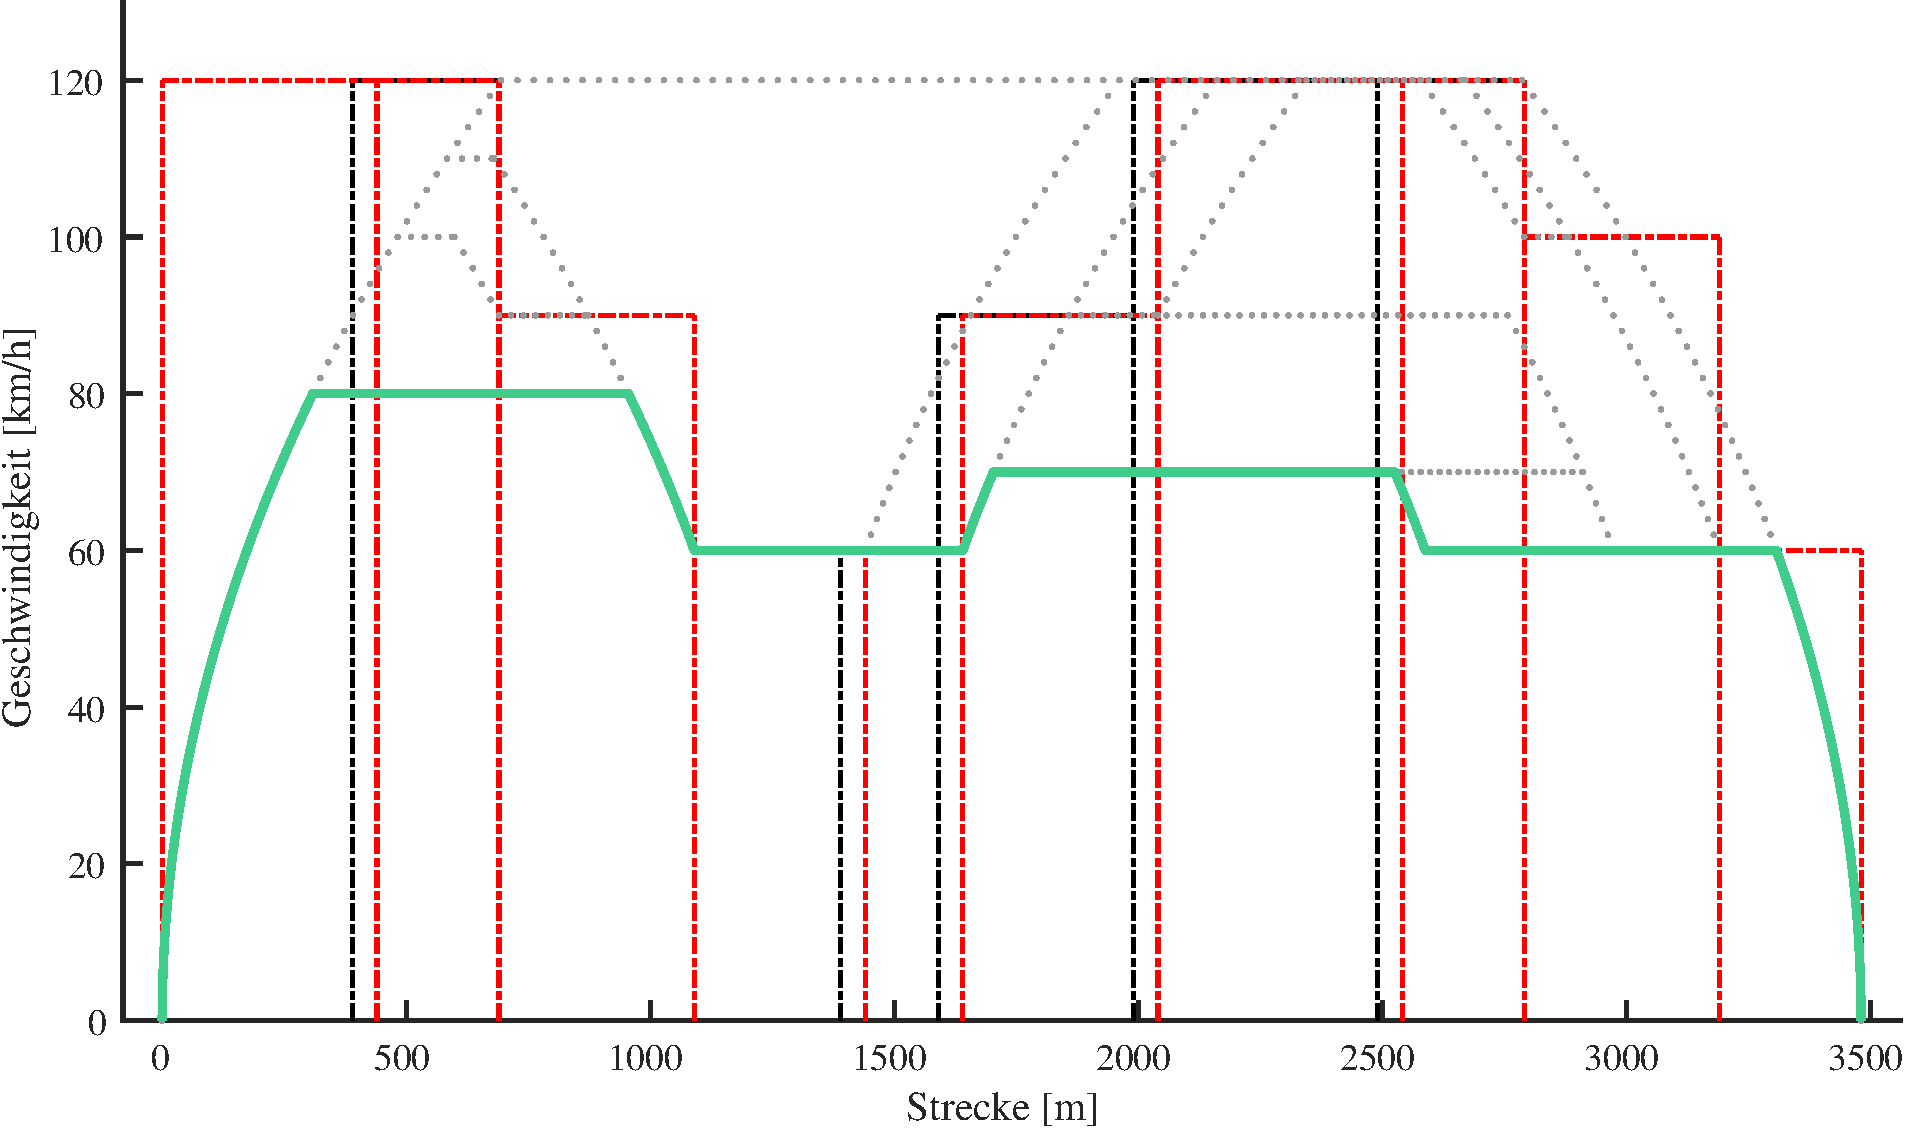
\includegraphics[width=\linewidth]{../images/matlab/it13.pdf}
  \caption{Finaler \Gls{fahrtverlauf}}
  \label{fig:it13}
\end{figure}
\subsection{Einleitung einer Gefahrenbremsung} \label{notbremsung}
Eine Gefahrenbremsung wird eingeleitet, sobald ein Fahrzeug bei einer sofortigen Verzögerung ein auf Halt stehendes Signal überfahren würde, in einem Infrastruktur-Abschnitt die zulässige Höchstgeschwindigkeit überschreiten würde oder an dem nächsten planmäßigen Halt nicht rechtzeitig zum stehen kommen würde. Bei einer Gefahrenbremsung wird mit einer Notbremsverzögerung von 2$m/s^2$ abgebremst. Dieser Wert kann in der Datei \textit{globalVariables.php} über die Variable \textit{\$globalNotverzoegerung} angepasst werden. Für eine möglichst realitätsnahe Simulation einer Gefahrenbremsung, bei der das Risiko für Fahrzeugschäden möglichst gering ist, wurde sich dafür entschieden, dass die Fahrzeuge, wenn sie an der Gefahrenstelle eine Geschwindigkeit haben, für die gilt: $v\geq10km/h$, nach der Geschwindigkeit von 10$km/h$ direkt die Geschwindigkeit von 0$km/h$ übermittelt bekommen. Dadurch wird bei der Berechnung einer Gefahrenbremsung zwischen drei Fällen unterschieden:
\begin{enumerate}
\item Fahrzeug hält mit der Notbremsverzögerung vor der Gefahrenstelle
\item Fahrzeug hat bei der Gefahrenstelle eine Geschwindigkeit von $v<10km/h$
\item Fahrzeug hat bei der Gefahrenstelle eine Geschwindigkeit von $v\geq10km/h$
\end{enumerate}
Für die Überprüfung, ob das Fahrzeug mit der Notbremsverzögerung vor der Gefahrenstelle zum Stehen kommt, wird mittels der Funktion \textit{getBrakeDistance$($$)$} der Bremsweg ($s_{Bremsweg}$) berechnet und mit der Distanz zur Gefahrenstelle ($s_{Gefahrenstelle}$) verglichen. Sollte für den Bremsweg gelten: $s_{Bremsweg}\leq s_{Gefahrenstelle}$, wird das Fahrzeug die Gefahrenbremsung einleiten und in 2$km/h$-Schritten auf 0$km/h$ abbremsen. In dem Fall, dass der Bremsweg länger als die Strecke bis zur Gefahrenstelle ist, wird überprüft, welche Geschwindigkeit das Fahrzeug an der Gefahrenstelle hat. Für diese Berechnung wird die Gleichung \ref{eq:gefahrenbremsung} aus dem Kapitel \ref{formula} verwendet. Sollte das Fahrzeug an der Gefahrenstelle eine Geschwindigkeit von $v\geq10km/h$ haben, bremst das Fahrzeug in 2$km/h$-Schritten auf 10$km/h$ ab und bekommt nach der Übermittlung der 10$km/h$ direkt 0$km/h$ übergeben. In dem Fall, dass das Fahrzeug an der Gefahrenstelle langsamer als 10$km/h$ ist, bremst das Fahrzeug wie im 1. Fall in 2$km/h$-Schritten auf 0$km/h$ ab. Bei einer Gefahrenbremsung bekommt das jeweilige Fahrzeug eine Fehlermeldung übermittelt und wird nicht weiterfahren. Das liegt daran, dass durch die Gefahrenbremsung keine genaue Positionsbestimmung vorgenommen werden kann. Damit das Fahrzeug wieder seinen Fahrtbetrieb aufnehmen kann, muss das Fahrzeug händisch von der Anlage genommen werden, gewartet werden, bis die Fahrzeugsteuerung das Entfernen registriert hat und wieder neu positioniert werden.